\documentclass[../main.tex]{subfiles}
\graphicspath{{\subfix{..}}}

\begin{document}
\chapter{Machine learning: Introduction to the methods and algorithms used in this thesis}
\label{sec:ml}

\epigraph{``I have the shape of a human being and organs equivalent to those of a human being. My organs, in fact, are identical to some of those in a prosthetized human being. I have contributed artistically, literally, and scientifically to human culture as much as any human being now alive. What more can one ask?''}{Isaac Asimov, The Complete Robot }

\minitoc

Machine Learning (ML) and more specifically Neural Network (NN) are families of data-driven algorithms. They are used in a wide variety of domains including natural language processing, computer vision, speech recognition and, the subject of this thesis, scientific studies.

Machine learning models aim to learn underlying patterns from finite datasets in order to make general predictions or classifications.
For example, in our case, it could be an algorithm that would differentiate the nature of a particle interacting in the liquid scintillator, between a positron and an electron, based on the readout charge and time $(Q, t)$ of the 17612 LPMT of the JUNO experiment. During a first training phase, it would learn the discriminative features between the two in the 35224-dimensional charge and time distribution, built from samples of $e^+$ and $e^-$ events.

It extracts essential features from a highly complex and multi-dimensional dataset that describe the physical interactions: a three body energy deposition (the positron and two annihilation gammas) and the single deposit from an electron.

Ideally, the algorithm would learn to recognize those informations on its own, regardless of the input size and complexity. In practice, however, these algorithms are guided by human design through their architectures and training conditions. We can still hope that they an use more thoroughly the detector informations while traditional methods are often subject to assumptions or simplifications to make the task easier (see for instance the algorithm in Section \ref{sec:juno:reco}).

The role of machine learning algorithms has expanded rapidly in the past decade, either as the main or secondary algorithm for a wide variety of tasks: event reconstruction, event classification, waveform reconstruction and so on. In particular in domains where the underlying physic and detector processes are complex and highly dimensional, and when large amount of data must be processed quickly.

This chapter present an overview of the different kind of machine learning methods and neural networks that will be discussed in this thesis.

\section{Core concepts in machine learning and neural networks}

In this section, we discuss the core concepts in machine learning that will be used thorough this thesis. We place particular emphasis on Neural Networks, as it's the family of the algorithms described in chapters \ref{sec:jcnn}, \ref{sec:jgnn} and \ref{sec:janne}.

\subsection{Boosted Decision Tree (BDT)}
\label{sec:ml:bdt}

One of the most classic machine learning algorithm used in particle physics is Boosted Decision Tree (BDT) \cite{breiman_classification_2017} (or more recently Gradient Boosting Machine \cite{friedman_greedy_2001}).

BDTs operate by making a series of decisions based on a set of input features, with each decision represented as a node in the tree.
Each decision point, or node, takes its decision based on a set of trainable parameters leading to a subtree of decisions. The process is repeated until it reach the final node, yielding the prediction. A simplistic example is given in Figure \ref{fig:ml:bdt}.

\begin{figure}
  \centering
  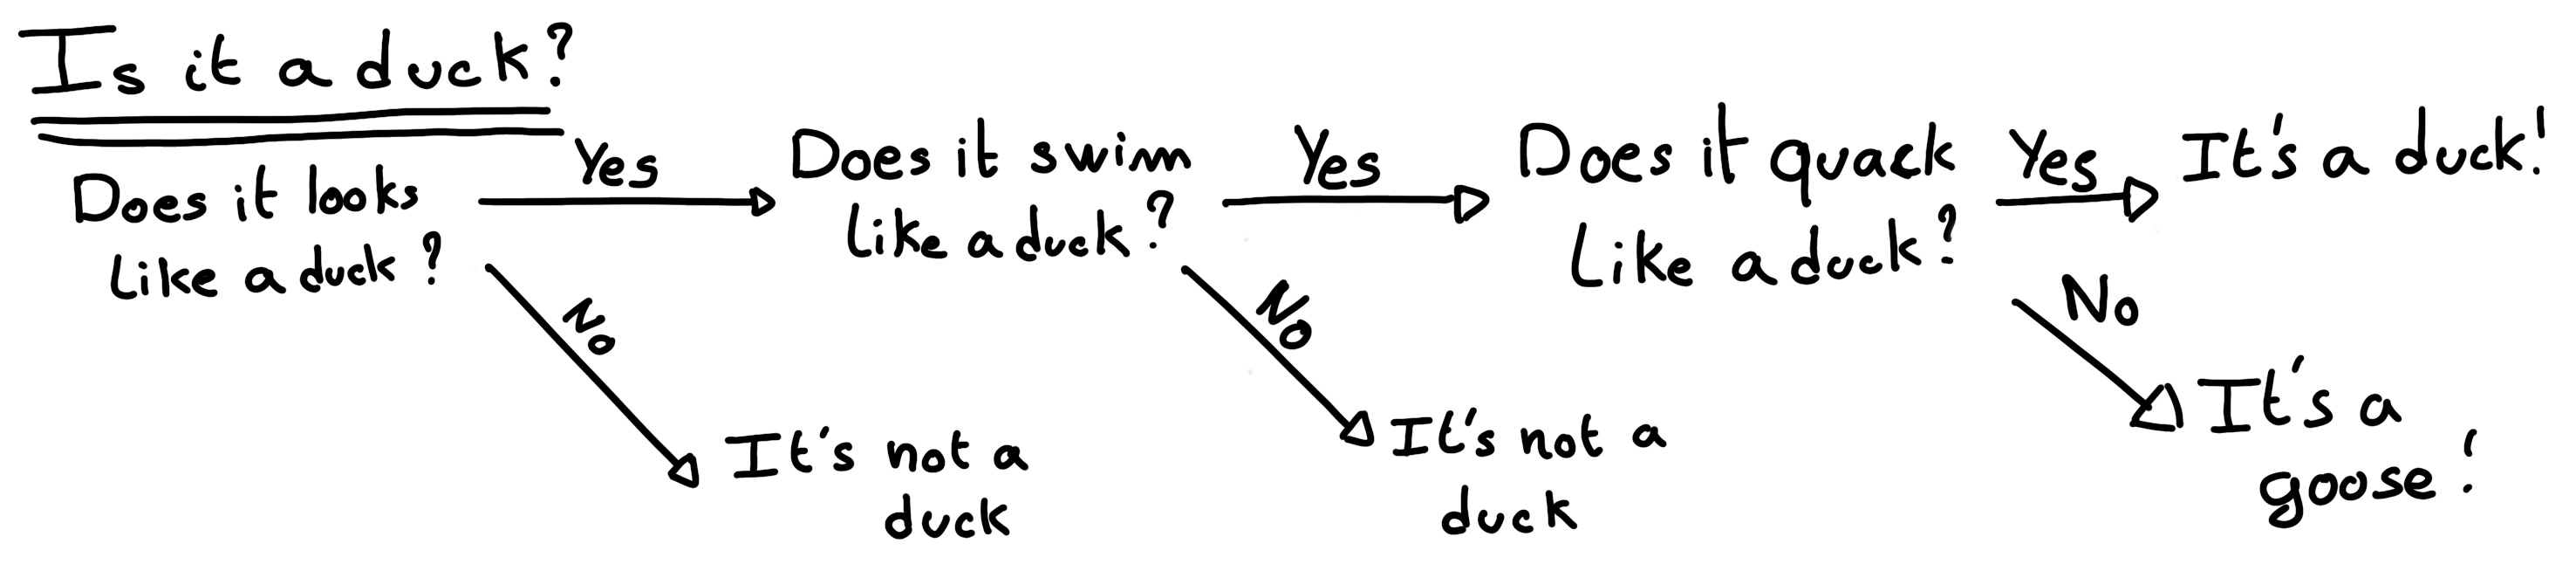
\includegraphics[width=\linewidth]{images/ml/Bdt.jpg}
  \caption{Example of a BDT that determine if the given object is a duck}
  \label{fig:ml:bdt}
\end{figure}

The training procedure followes a reward-based approach where the algorithm predictions are compared to the true outcomes.
During the training phase the prediction of the BDT is compared to a known truth about the data. The score is then used to backpropagate corrections to the parameters of the tree. Modern BDT use gradient boosting where the gradient of the loss is calculated for each of the BDT parameters. Following the gradient descent, we can reach the, hopefully, global minima of the loss for our set of parameters.

\subsection{Artificial Neural Network (NN)}
\label{sec:ml:nn}

One of the modern ML family is the Neural Network, historical name as their design was inspired by the behaviour of biological neurons in the brain.
\begin{figure}[ht]
  \centering
  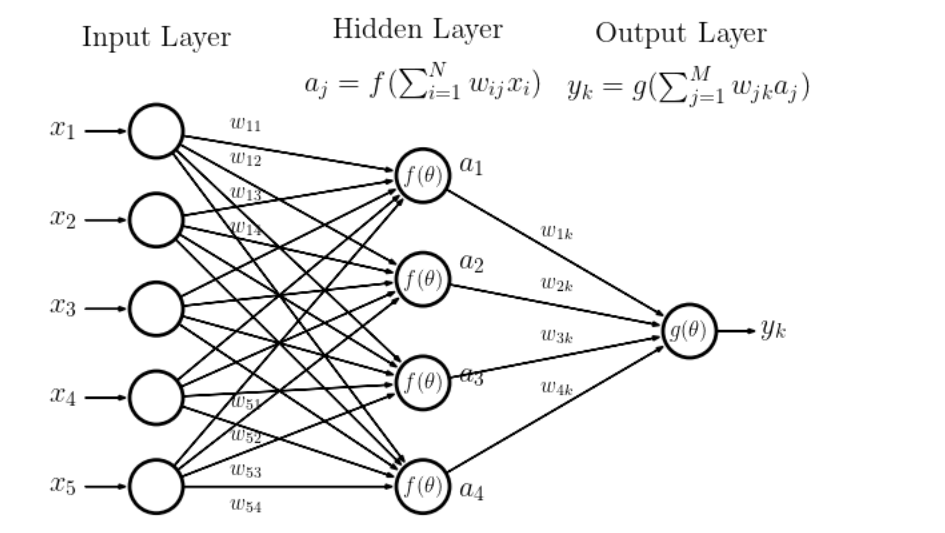
\includegraphics[height=6cm]{images/ml/nn_explications.png}
  \caption{Schema of a simple neural network}
  \label{fig:ml:schema_nn}
\end{figure}
As schematized in Figure \ref{fig:ml:schema_nn}, the input, output and steps inside the NN is described as neuron \textit{layers}. The neurons of the layers take as input a set of values from the preceding layer, here the $a_i$ takes every informations of the $x_i$ input layer, and aggregate those values following learnable \textit{parameters} $w_{ij}$. In the example in Figure \ref{fig:ml:schema_nn}, fully connected layers are used, meaning that each neuron in one layer is connected to every neuron in the previous layer.

The aggregation procedure is core of defining the architecture of the NN. The different architectures used in this thesis will be discussed in Section \ref{sec:ml:architecture}. The process is repeated until reaching the output layer.

For example, let's take the network in Figure \ref{fig:ml:schema_nn} and say that $a_1$, $a_2$ and $a_3$ are the neurons of the output layer. We try to produce a vertex reconstruction algorithm that will approach the charge barycentre. Let's limit the input $x_i$ to the charge of the $i$th PMT, one of the solution is to aggregate on $a_1$ the $x$ coordinate of the barycenter. The network would thus adapt the $w_{i1}$ parameters so they correspond to the $x$ coordinates of the $i$th PMT. Same for the $y$ and $z$ coordinate on $a_2$ and $a_3$ respectively.

The layers used in the example above are designated as \textit{Fully connected} layers, where every neurons of the layer is connected to the every neurons of the preceding layer. The layer can be expressed using the Einstein summation and in bold the learnable parameters
\begin{equation}
  \label{eq:ml:fully-connected-simple}
  O_{j} = I_{i} + \bm{W}_{j}^{i}
\end{equation}
where $O_{j}$ is the output neurons vector (the $a_i$), $I_{i}$ is the preceding layer neurons vector (the $x_i$) and $\bm{W}$ is the parameters, or weights, matrix (composed of the $w_{ij}$).
In practice, this fully connected layer is often adjoined a bias $\bm{B}$ and an \textit{activation function} $F$.
\begin{equation}
  \label{eq:ml:fully-connected}
  I_{j} = F(I_{i} \bm{W}_{j}^{i} + \bm{B}_j)
\end{equation}

This is the fundamental component of the Fully Connected Deep NN (FCDNN) family presented in Section \ref{sec:ml:fcdnn}.

This description of neural networks as layers introduce the principles of \textit{depth} and \textit{width}, the number of layers in the NN and the number of neurons in each layer respectively. Those quantities that not directly used for the computation of the results but describes the NN or its training are designated as \textit{hyperparameters}.

Now we just need to adapt the parameters so that this network learn that $w_{ij}$ are the PMT coordinate. We describe the space produced by the parameters of the network as the \textit{parameter phase space} or \textit{latent space}. The optimization of the network and exploration of this phase space is done through training over a \textit{training dataset} as described in next section.

\subsection{Training procedure}
\label{sec:ml:train}

To adapt the parameters we need an object that describe how well the network perform. This is the \textit{loss} of our neural networks $\mathcal{L}$. In our barycenter example, it could be the distance between the reconstructed and real barycenter. Using this metric we can adjust the parameters of our network.

Depending if we try to minimize or maximize it, it need to posses a minima or a maxima. For example when doing \textit{regression}, i.e. produce a scalar result like the coordinates of a barycenter, a common loss is the Mean Square Error (MSE). Let $i$ be our dataset, the $N$ events considered for training, $y_i$ be the target scalar, the barycenter positions of each events, $x_i$ the input data, the charge vector, and $f(x_i, \bm{\theta})$ the result of the network. The network here is modelled by $f$, and its parameter $\bm{\theta}$
\begin{equation}
  \mathcal{L} \equiv MSE = \frac{1}{N} \sum_i^N (y_i - f(x_i, \bm{\theta}))^2
\end{equation}
Another common loss function is the Mean Absolute Error (MAE)
\begin{equation}
  \mathcal{L} \equiv MAE = \frac{1}{N} \sum_i^N |y_i - f(x_i, \bm{\theta})|
\end{equation}

We see that those loss function possess a minima when $f(x_i, \bm{\theta}) = y_i$.


Modern neural networks typically use gradient descent to optimize their parameters by minimizing the loss function. The gradient of the parameter $\bm{w}$, designated in literature as $\bm{\theta}$, with respect of the loss function $\mathcal{L}$ is subtracted each optimisation step $t$
\begin{equation}
  \bm{\theta}_{t+1} = \bm{\theta}_t - \frac{\partial \mathcal{L}}{\partial \bm{\theta}}
\end{equation}
This induce $\mathcal{L}$  needs to be differentiable with respect to $\bm{\theta}$, thus the layers and their activation functions also need to be differentiable. This simple gradient descent, designated as Stochastic Gradient Descent (SGD), can be extended with first and second order momentums like in the Adam optimizer \cite{kingma_adam_2017}. More details about the optimizers can be found in Section \ref{sec:ml:optim}.

\subsubsection{Training lifecycle}

The training process of neural networks can vary depending on the application and dataset, but in this thesis, we follow a standard approach. As shown in Fig. \ref{fig:ml:lifecycle}, training is organized into \textit{epochs}, each of which consists of several \textit{steps}. During each step, the neural network optimizes its parameters using a \textit{batch}, a subset of the entire training dataset.

\begin{figure}[ht]
  \centering
  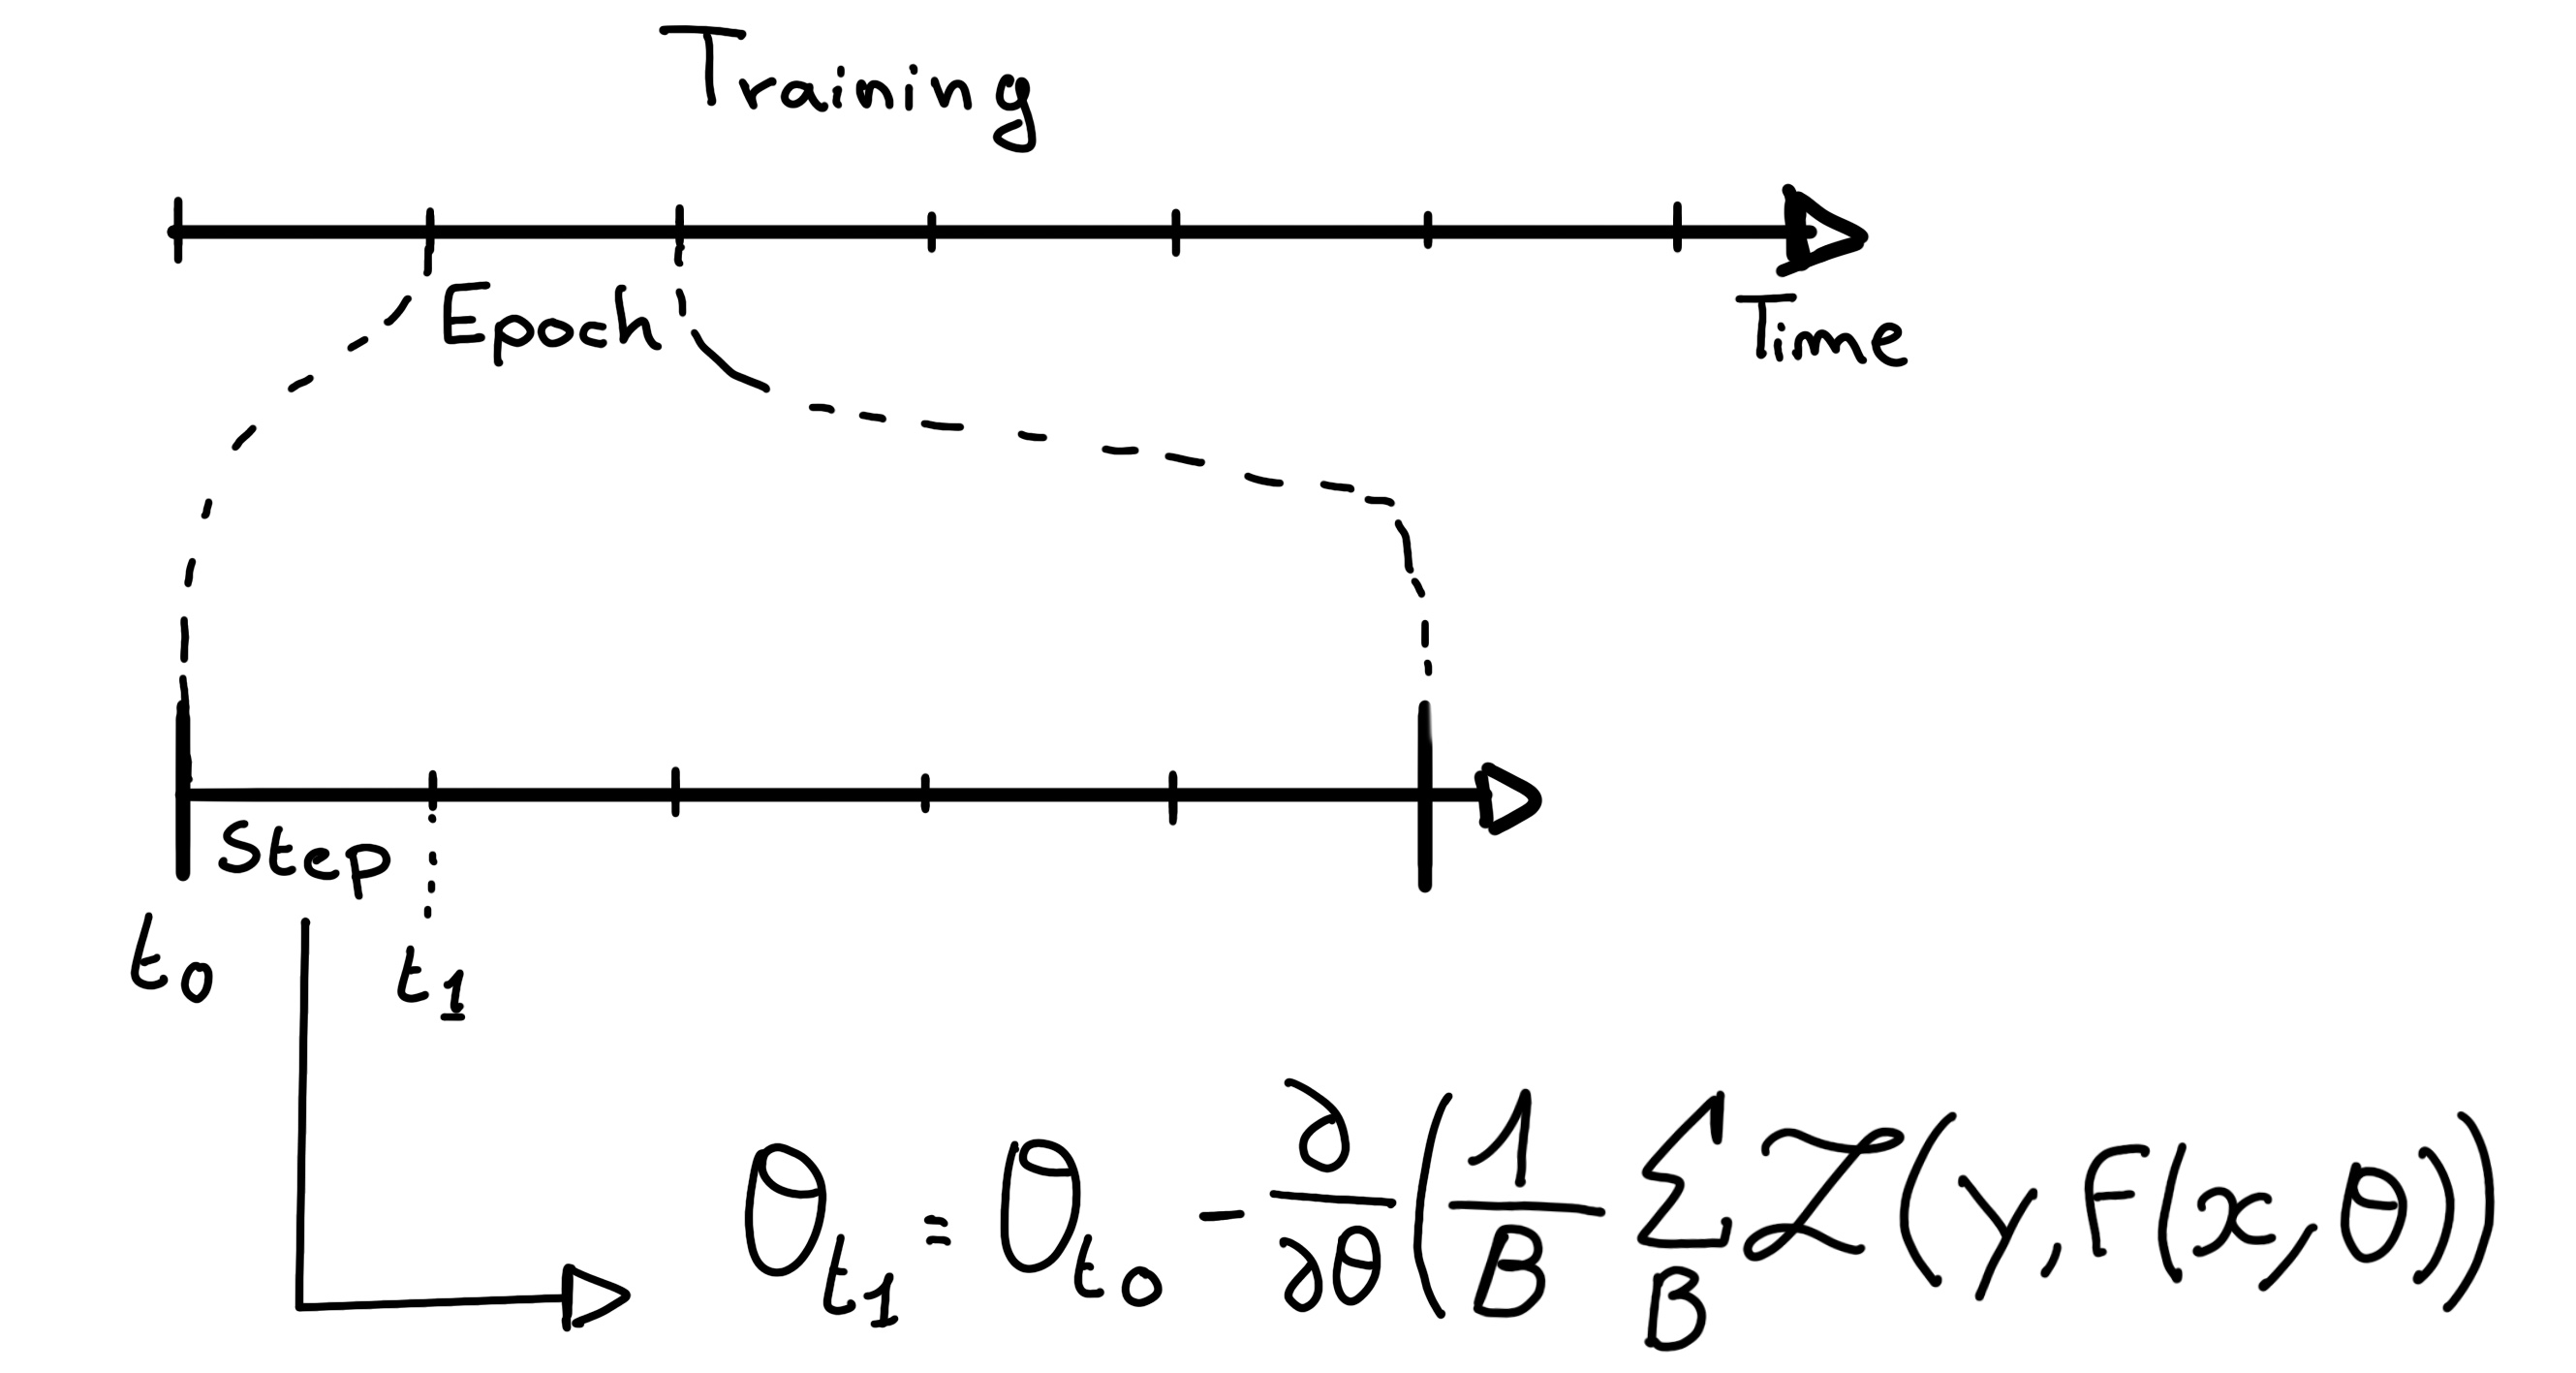
\includegraphics[height=6cm]{images/ml/lifecycle.jpg}
  \caption{Illustration of the training lifecycle}
  \label{fig:ml:lifecycle}
\end{figure}

The ideal batch size, meaning the number of events in each batch, would encompass the entire dataset to avoid bias introduced by sub-sample specificity. However, in large-scale experiments like JUNO, the batch size is often constrained by memory limitations due to the massive volume of data generated by the photomultiplier tubes (PMTs). Balancing batch size with memory capacity is crucial to ensure efficient and accurate training.

At the end of each epoch, the neural network is evaluated on a validation dataset, which is not used during training. This dataset serves as a reference to assess the network's performance and to monitor for signs of overfitting. In JUNO, this is critical because the model needs to generalize well to unseen experimental data and avoid overfitting to noise in the training set (see Section \ref{sec:ml:pitfall}).

Hyperparameters that can be optimized during the training can be optimized at each epoch, for example the learning rate, or each step, the optimizer momentum for example.

There is not really a typical number of epochs or steps for the training. The number steps can be defined such as in one epoch, the NN see the entirety of the dataset but the number of steps and epochs are hyperparameters that are optimized over the each subsequent training. We adjust them by looking at the loss evolution profile over time.

Most training are started with a fixed number of epochs, i.e. from what we've seen from precedent training, the network stop learning, the loss is constant, after $N$ epoch so we run the training for $N+\delta$ epochs to see if the modification brings improvements to the loss profile.
We can implement \textit{early stopping policies} to halt training if certain conditions are met, such as a sudden increase in loss or when the loss plateaus. However, for the JUNO experiment, where training time is not a strict limitation, early stopping is less critical, though it may still be useful to prevent overfitting in some cases

\subsubsection{The optimizer}
\label{sec:ml:optim}

As briefly introduced at the beginning of this section, the parameters of the neural network are optimized using the gradient descent method. We compute the gradient of the mean loss over the batch with respect of each parameters and we update the parameters in accord to minimize the loss. The  gradient is computed backward from the loss up to the first layer parameters using the chain rule, in this case with only one parameter at each step for simplicity:
\begin{equation}
  \label{eq:ml:backward}
  \frac{\partial \mathcal{L}}{\partial \theta_1} = \frac{\partial \theta_2}{\partial \theta_1} \frac{\partial \mathcal{L}}{\partial \theta_2} = \frac{\partial \theta_2}{\partial \theta_1} \frac{\partial \theta_3}{\partial \theta_2} \frac{\partial \mathcal{L}}{\partial \theta_3} = \frac{\partial \theta_2}{\partial \theta_1} \prod_{i=2}^{N-1} \frac{\partial \theta_{i+1}}{\partial \theta_i} \frac{\partial \mathcal{L}}{\partial \theta_N}
\end{equation}
where $\theta$ is a parameter, $i$ is the layer index. We see here that the gradient of the first layer is dependent of the gradient of all the following layers. Because the only value known at the start of the optimization procedure is $\mathcal{L}$ we compute $\frac{\partial \mathcal{L}}{\partial \theta_N}$ then, $\frac{\partial \theta_{N}}{\partial \theta_{N-1}}$, etc... This is called the \textit{backward propagation}.

This update of the parameters is done following an optimizer policy. Those optimizers depends on hyperparameters. The ones used in this thesis are:

\begin{enumerate}
  \item Stochastic Gradient Descent (SGD).
    A simple but widely used optimizer that relies on one key hyperparameter, the learning rate (LR) / $\lambda$. It update each step the parameters $\theta$ following
    \begin{equation}
      \theta_{t+1} = \theta_t - \lambda \frac{\partial \mathcal{L}}{\partial \theta}\bigg|_{\theta_t}
    \end{equation}
    where $t$ is the step index. It is a powerful optimizer but is very sensible to local minima of the loss in the parameters phase space as illustrated in Figure \ref{fig:ml:sgd}.

  \item Adam Optimizer \cite{kingma_adam_2017}. The concept is, in short, to have and SGD but with momentum. Adam possess two momentum $m(\beta_1)$ and $v(\beta_2)$ which are respectively proportional to $\frac{\partial \mathcal{L}}{\partial \theta}$ and $(\frac{\partial \mathcal{L}}{\partial \theta})^2$. $\beta_1$ and $\beta_2$ are hyperparameters that dictate the moment update at each optimization step. The parameters are then upgraded following \begin{align}
      m_{t+1} &= \beta_1 m_t + (1 - \beta_1) \frac{\partial \mathcal{L}}{\partial \theta} \\
      v_{t+1} &= \beta_2 v_t + (1 - \beta_2) \bigg(\frac{\partial \mathcal{L}}{\partial \theta}\bigg)^2 \\
      \theta_{t+1} &= \theta_{t} - \lambda \frac{m_{t+1}}{\sqrt{v_{t+1}} + \epsilon}
    \end{align}
    where $\epsilon$ is a small number to prevent divergence when $v$ is close to 0. These momentums allow to overcome small local minima in the parameters phase. Imagine ball going down a slope as illustrated in \ref{fig:ml:sgd}, if you ignore the stored momentum you get SGD and get stuck as on the left plot. Now if you consider the momentum you get over the hill and end up in the global minima.
\end{enumerate}

\begin{figure}
  \centering
  \begin{subfigure}[t]{0.48\linewidth}
    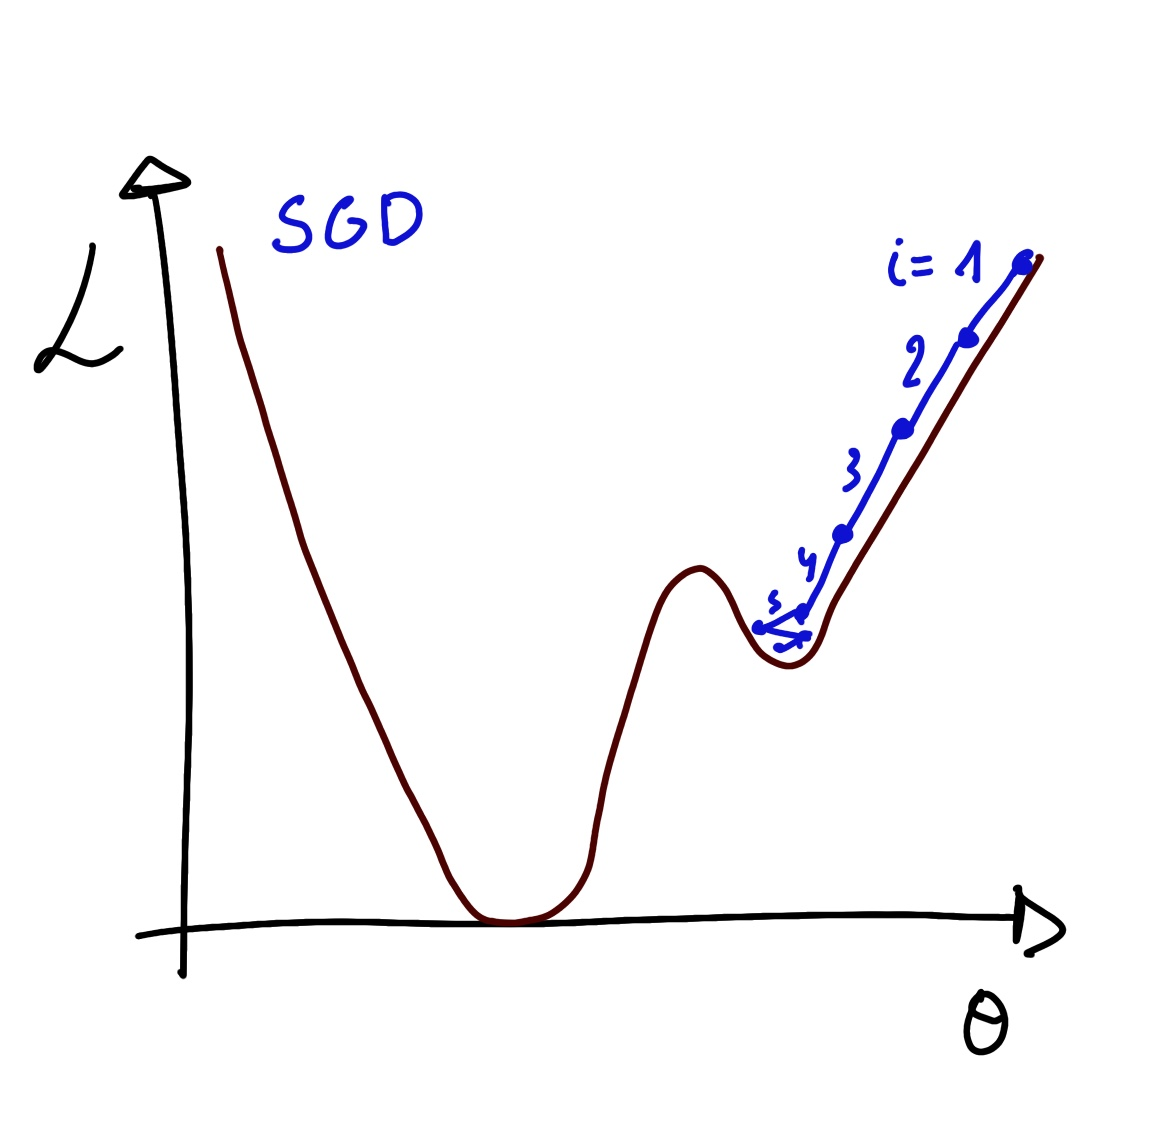
\includegraphics[height=6cm]{images/ml/sgd.jpg}
    \caption{Illustration of SGD falling into a local minima}
    \label{fig:ml:sgd}
  \end{subfigure}
  \hfill
  \begin{subfigure}[t]{0.48\linewidth}
    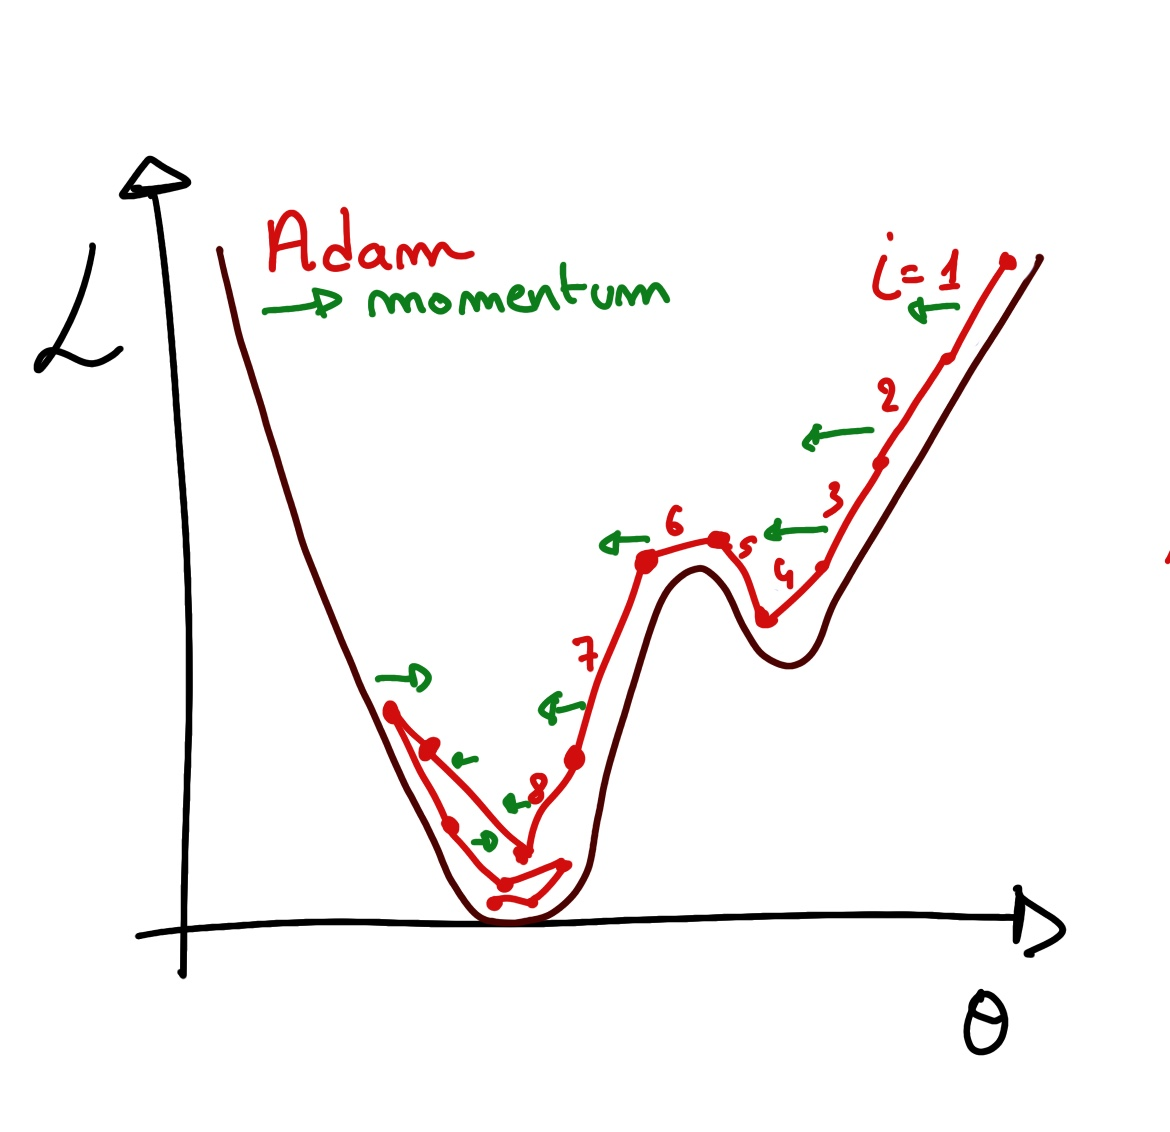
\includegraphics[height=6cm]{images/ml/Adam.jpg}
    \caption{Illustration of the Adam momentum allowing it to overcome local minima}
    \label{fig:ml:adam}
  \end{subfigure}
  \caption{}
\end{figure}

\subsubsection{Learning Rate (LR) Schedules}

The learning rate plays a crucial role in determining how fast or slow the model converges. If the learning rate is too high (Fig. \ref{fig:ml:optims:mae}), the model may skip over the optimal solution, whereas a low learning rate (Fig. \ref{fig:ml:optims:mse}) can slow down the convergence process, leading to inefficient training. To address this, learning rate schedulers are employed.

Using a learning rate scheduler allows the optimizer to take larger steps in the early stages of training, where rapid learning is beneficial, and progressively smaller steps as the model approaches convergence. This strategy is especially useful in JUNO, where early learning from noisy data may require coarse adjustments, but fine-tuning is needed later to accurately capture subtle event characteristics.

\begin{figure}
  \centering
  \begin{subfigure}[t]{0.48\linewidth}
    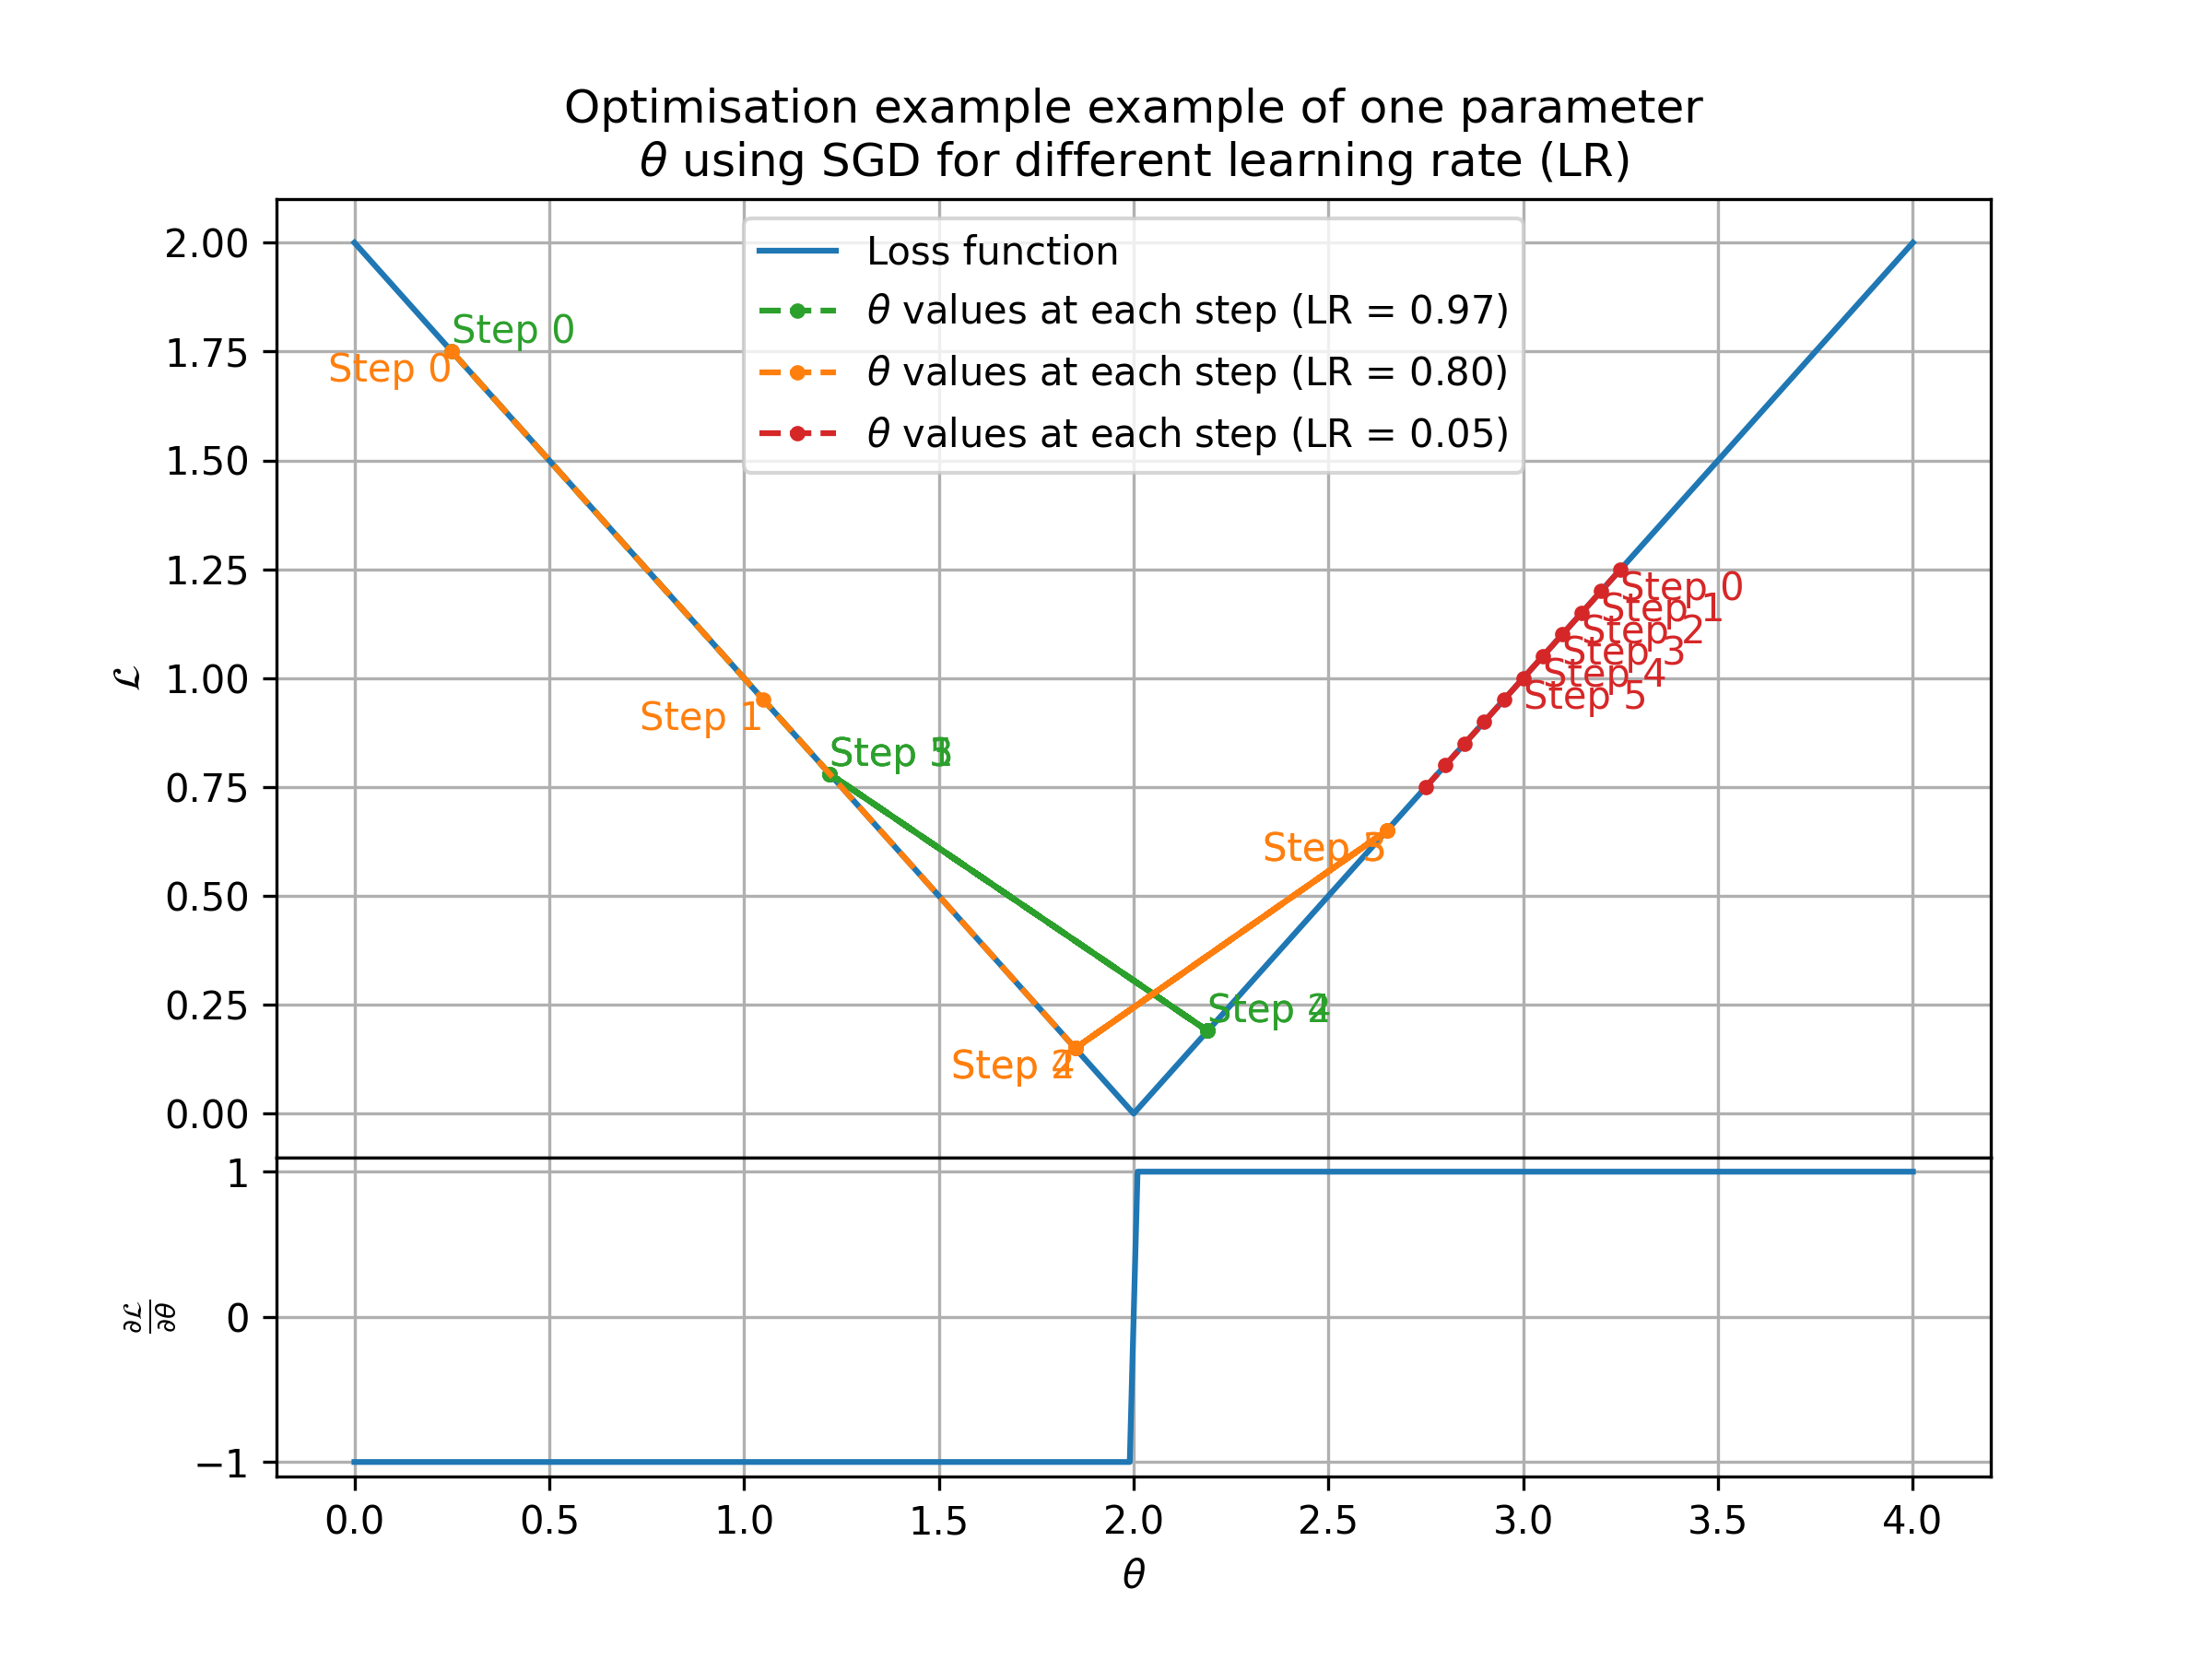
\includegraphics[height=6cm]{scripts/plots/MAE_illustration.png}
    \caption{Illustration of the SGD optimizer on one parameter $\theta$ on the MAE Loss. We see here that it has trouble reaching the minima due to the gradient being constant.}
    \label{fig:ml:optims:mae}
  \end{subfigure}
  \hfill
  \begin{subfigure}[t]{0.48\linewidth}
    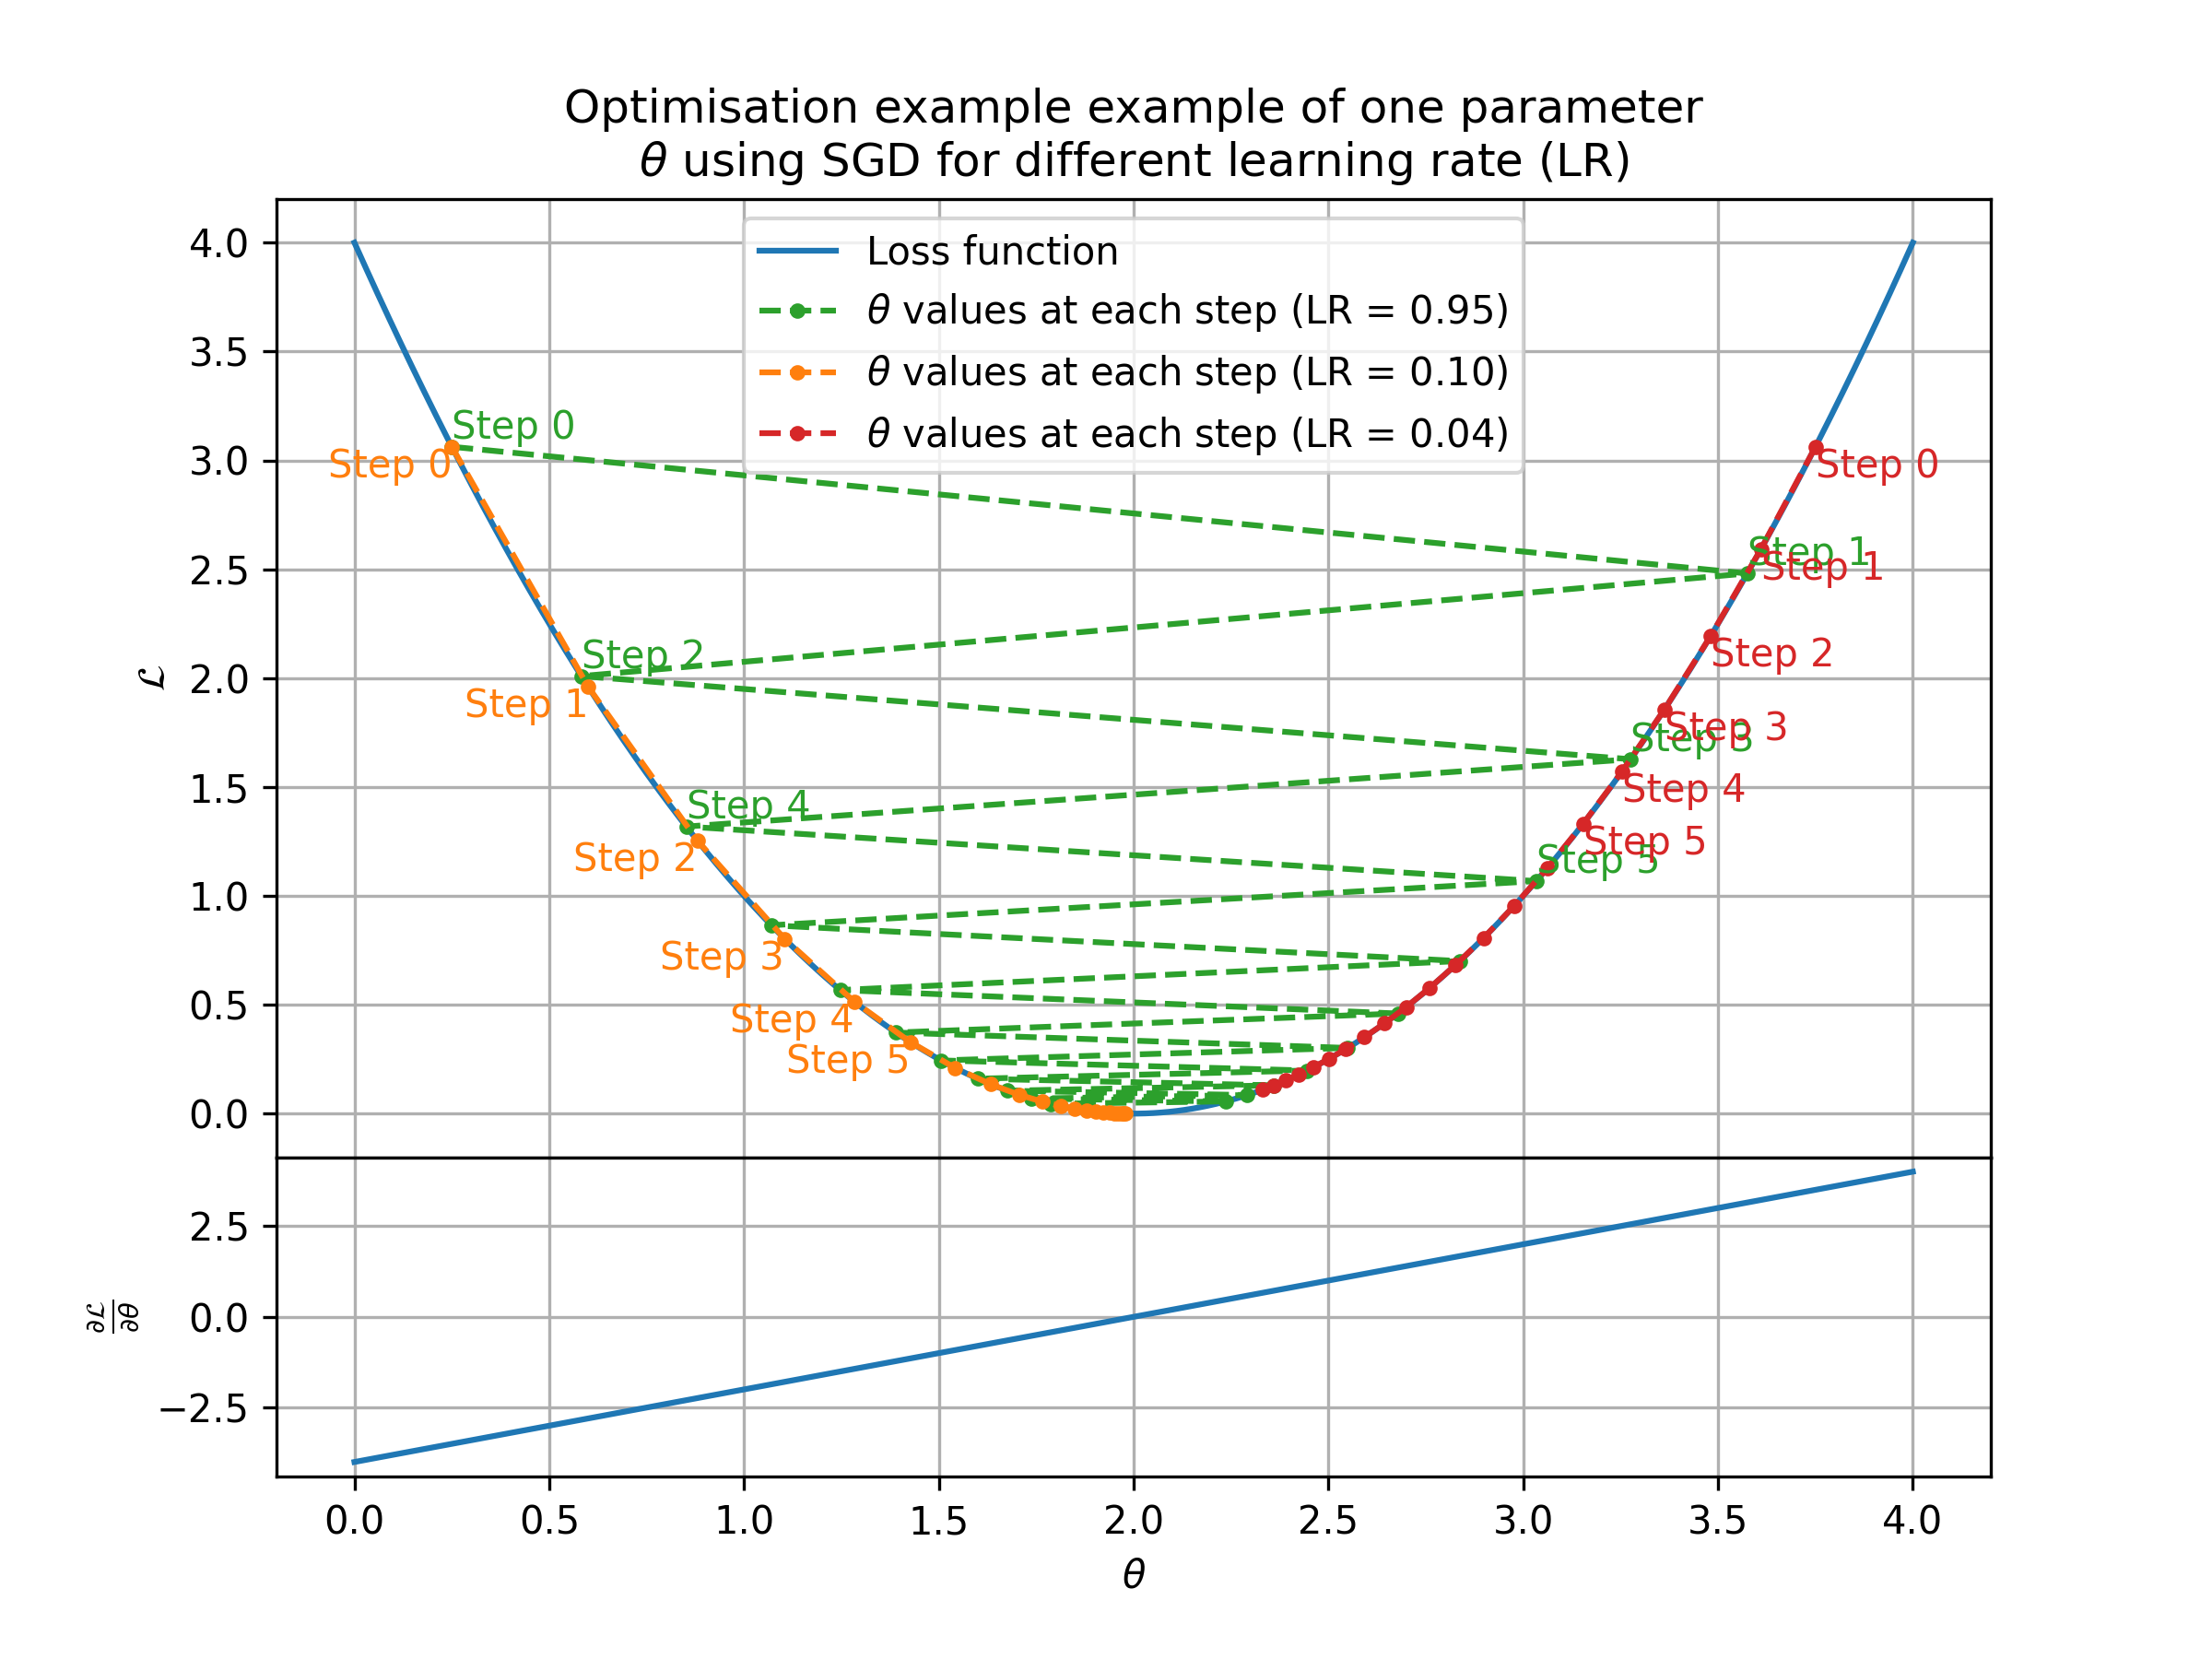
\includegraphics[height=6cm]{scripts/plots/MSE_illustration.png}
    \caption{Illustration of the SGD optimizer on one parameter $\theta$ on the MSE Loss. We see two different behavior: A smooth one (orange and red) when the LR is small enough and a more chaotic one when the LR is too high.}
    \label{fig:ml:optims:mse}
  \end{subfigure}
  \caption{Illustration of the SGD optimizer. In blue is the value of the loss function, orange, green and red are the path taken by the optimized parameter during the training for different LR.}
  \label{fig:ml:optims}
\end{figure}

Another policy that is often use is the save of the best model. In some situation, the loss value after each epoch will strongly oscillate or can even worsen. This policy allow us to keep the best version of the model attained during the training phase.

\subsection{Potential pitfalls}
\label{sec:ml:pitfall}

Apart from being stuck in local minima, there is also other behaviors and effects we want to prevent during training.

\subsubsection{Overtraining}

Overfitting occurs when a neural network memorizes specific details or noise from the training dataset rather than learning a general representation of the underlying data. This is common when the training dataset is small relative to the number of parameters in the network or when the dataset contains specific features that do not generalize well to unseen data. Additionally, training the network for too many epochs can exacerbate this issue. Figure \ref{fig:ml:overtraining} illustrates the impact of overfitting, where the model fits the training data too closely, compromising its ability to generalize.
To detect overfitting, techniques like monitoring the validation loss, early stopping, or employing cross-validation can be employed. In JUNO's context, managing overfitting is critical due to the large volume of data generated by the photomultiplier tubes (PMTs), which may include noise or other artifacts.

Overtraining can be fought in multiple ways, for example:
\begin{itemize}
  \item \textbf{More data}. By having more data in the training dataset, the network will not be able the specificities of every data.
  \item \textbf{Less parameters}. By reducing the number of parameters, we reduce the computing and learning capacities of the network. This will force it to fallback to generalist behaviours.
  \item \textbf{Dropout}. This technique implies to randomly set some neurons to 0, i.e. cutting the relation between two neurons in a layer. By doing this, we force the network to allocate more of its parameter to the features learning, preventing those parameters to be used for overtraining.
  \item \textbf{Early stopping}. During the training we monitor the network performance over a validation dataset. The network does not train on this dataset and thus cannot learn its specificities. If the loss on the training dataset diverge too much from the loss on the validation dataset, we can stop the training earlier to prevent it from overtraining.
\end{itemize}

\begin{figure}
  \centering
  \begin{subfigure}[t]{0.48\linewidth}
    \centering
    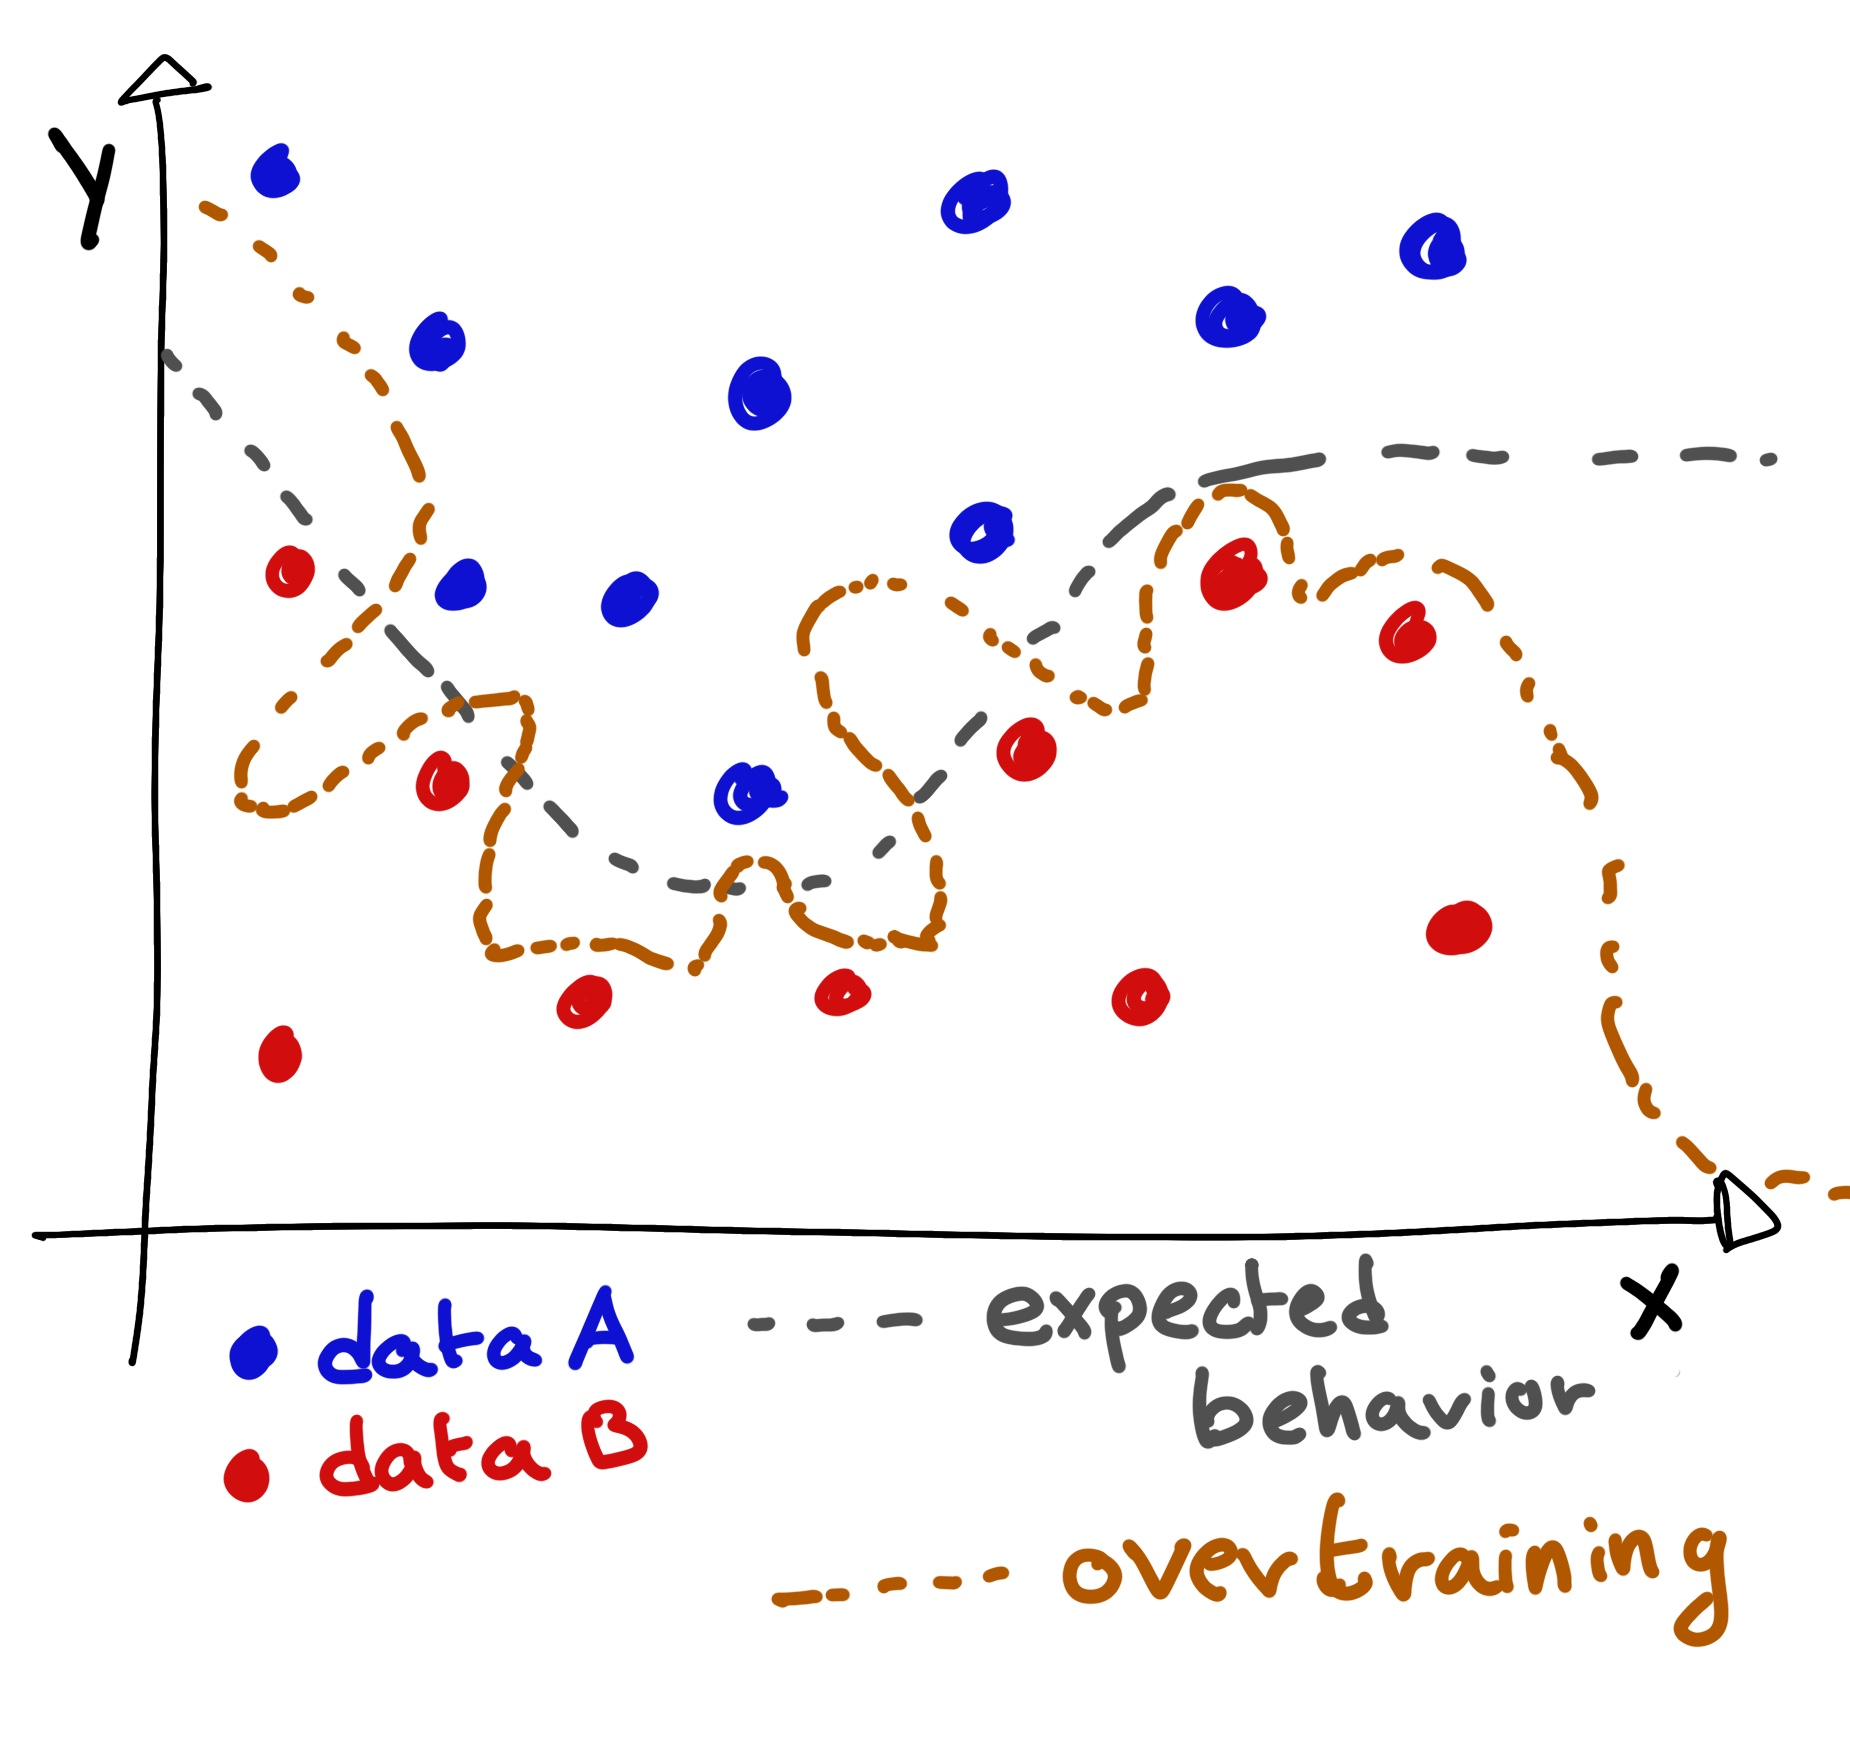
\includegraphics[height=6cm]{images/ml/overtraining.jpg}
    \caption{Illustration of overtraining. The task at hand is to determine depending on two input variable $x$ and $y$ if the data belong to the dataset $A$ or the dataset $B$. The expected boundary between the two dataset is represented in grey. A possible boundary learnt by overtraining is represented in brown.}
    \label{fig:ml:overtraining}
  \end{subfigure}
  \hfill
  \begin{subfigure}[t]{0.48\linewidth}
    \centering
    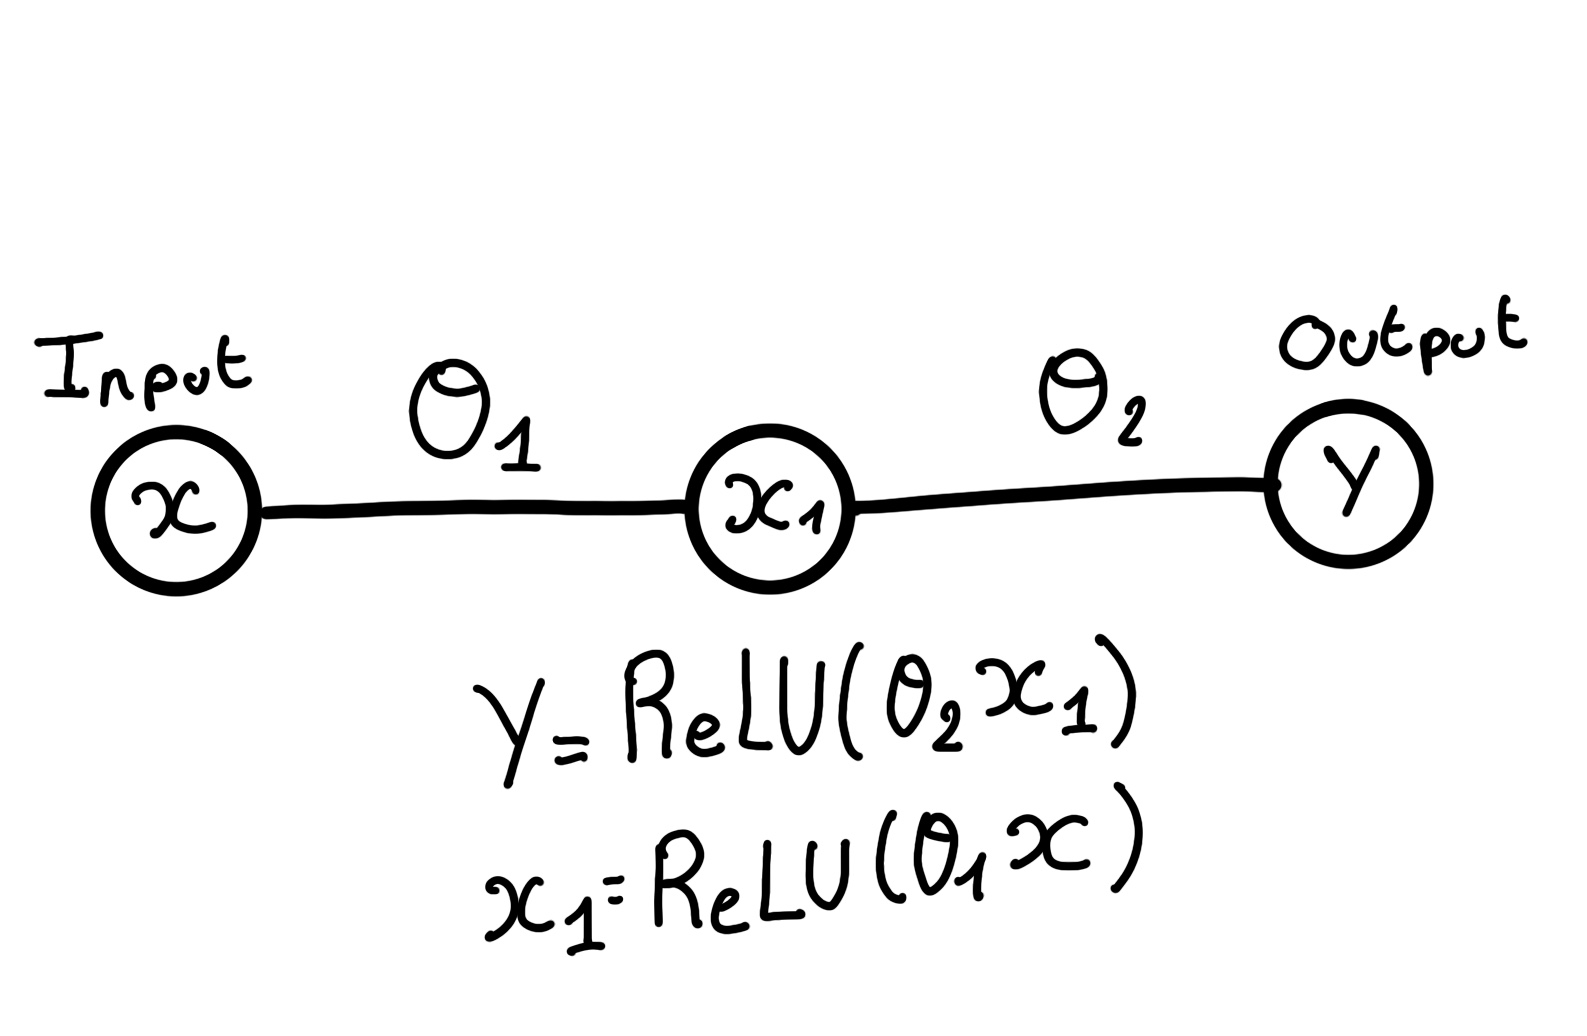
\includegraphics[height=6cm]{images/ml/vanishing_illus.jpg}
    \caption{Illustration of a very simple NN}
    \label{fig:ml:vanishing}
  \end{subfigure}
  \caption{}
\end{figure}

\subsubsection{Gradient vanishing}
Gradient vanishing is the effect of the gradient being so small for the early layers that the parameters are barely updated after each step. This cause the network to be unable to converge to the minima.

This comes from the way the gradient descent is calculated. Imagine a simple network composed of three fully connected layers: the input layer, a intermediate layer and the output layer. Let $L$ be the loss, $\theta_1$ the parameter between the input and the intermediate layer and $\theta_2$ the parameter between the intermediate and output layer. This network is schematized in Figure \ref{fig:ml:vanishing}.

The gradient for $\theta_1$ will be computed using the chain rule presented in equation \ref{eq:ml:backward}. Because $\theta_1$ depends on $\theta_2$, if the gradient of $\theta_2$ is small, so will be the gradient of $\theta_1$. Now if we would have much more layer, we can see how the subsequent multiplication of small gradients would lead to very small update of the parameters thus ``\textit{vanishing gradient}''.

Multiple actions can be taken to prevent this effect such as:
\begin{itemize}
  \item \textbf{Batch normalization}: In this case we apply a normalization layer that will normalize the data. It means that we transform the input variable $X$ into a variable $D$ which distribution follow $\langle D \rangle = 0$ and $\sigma D = 1$. This helps the parameters of the network to maintain an appropriate scale.
  \item \textbf{Residual Network (ResNet)} \cite{he_deep_2016}: Residual network is a technique for neural network in which, instead of just sequentially feeding the results of each layer to the next one, you compute a residual over the input data. This technique is illustrated in Figure \ref{fig:ml:resnet}. The reference \cite{he_deep_2016} show empirical evidence of its relevance.
\end{itemize}


\begin{figure}[ht]
  \centering
  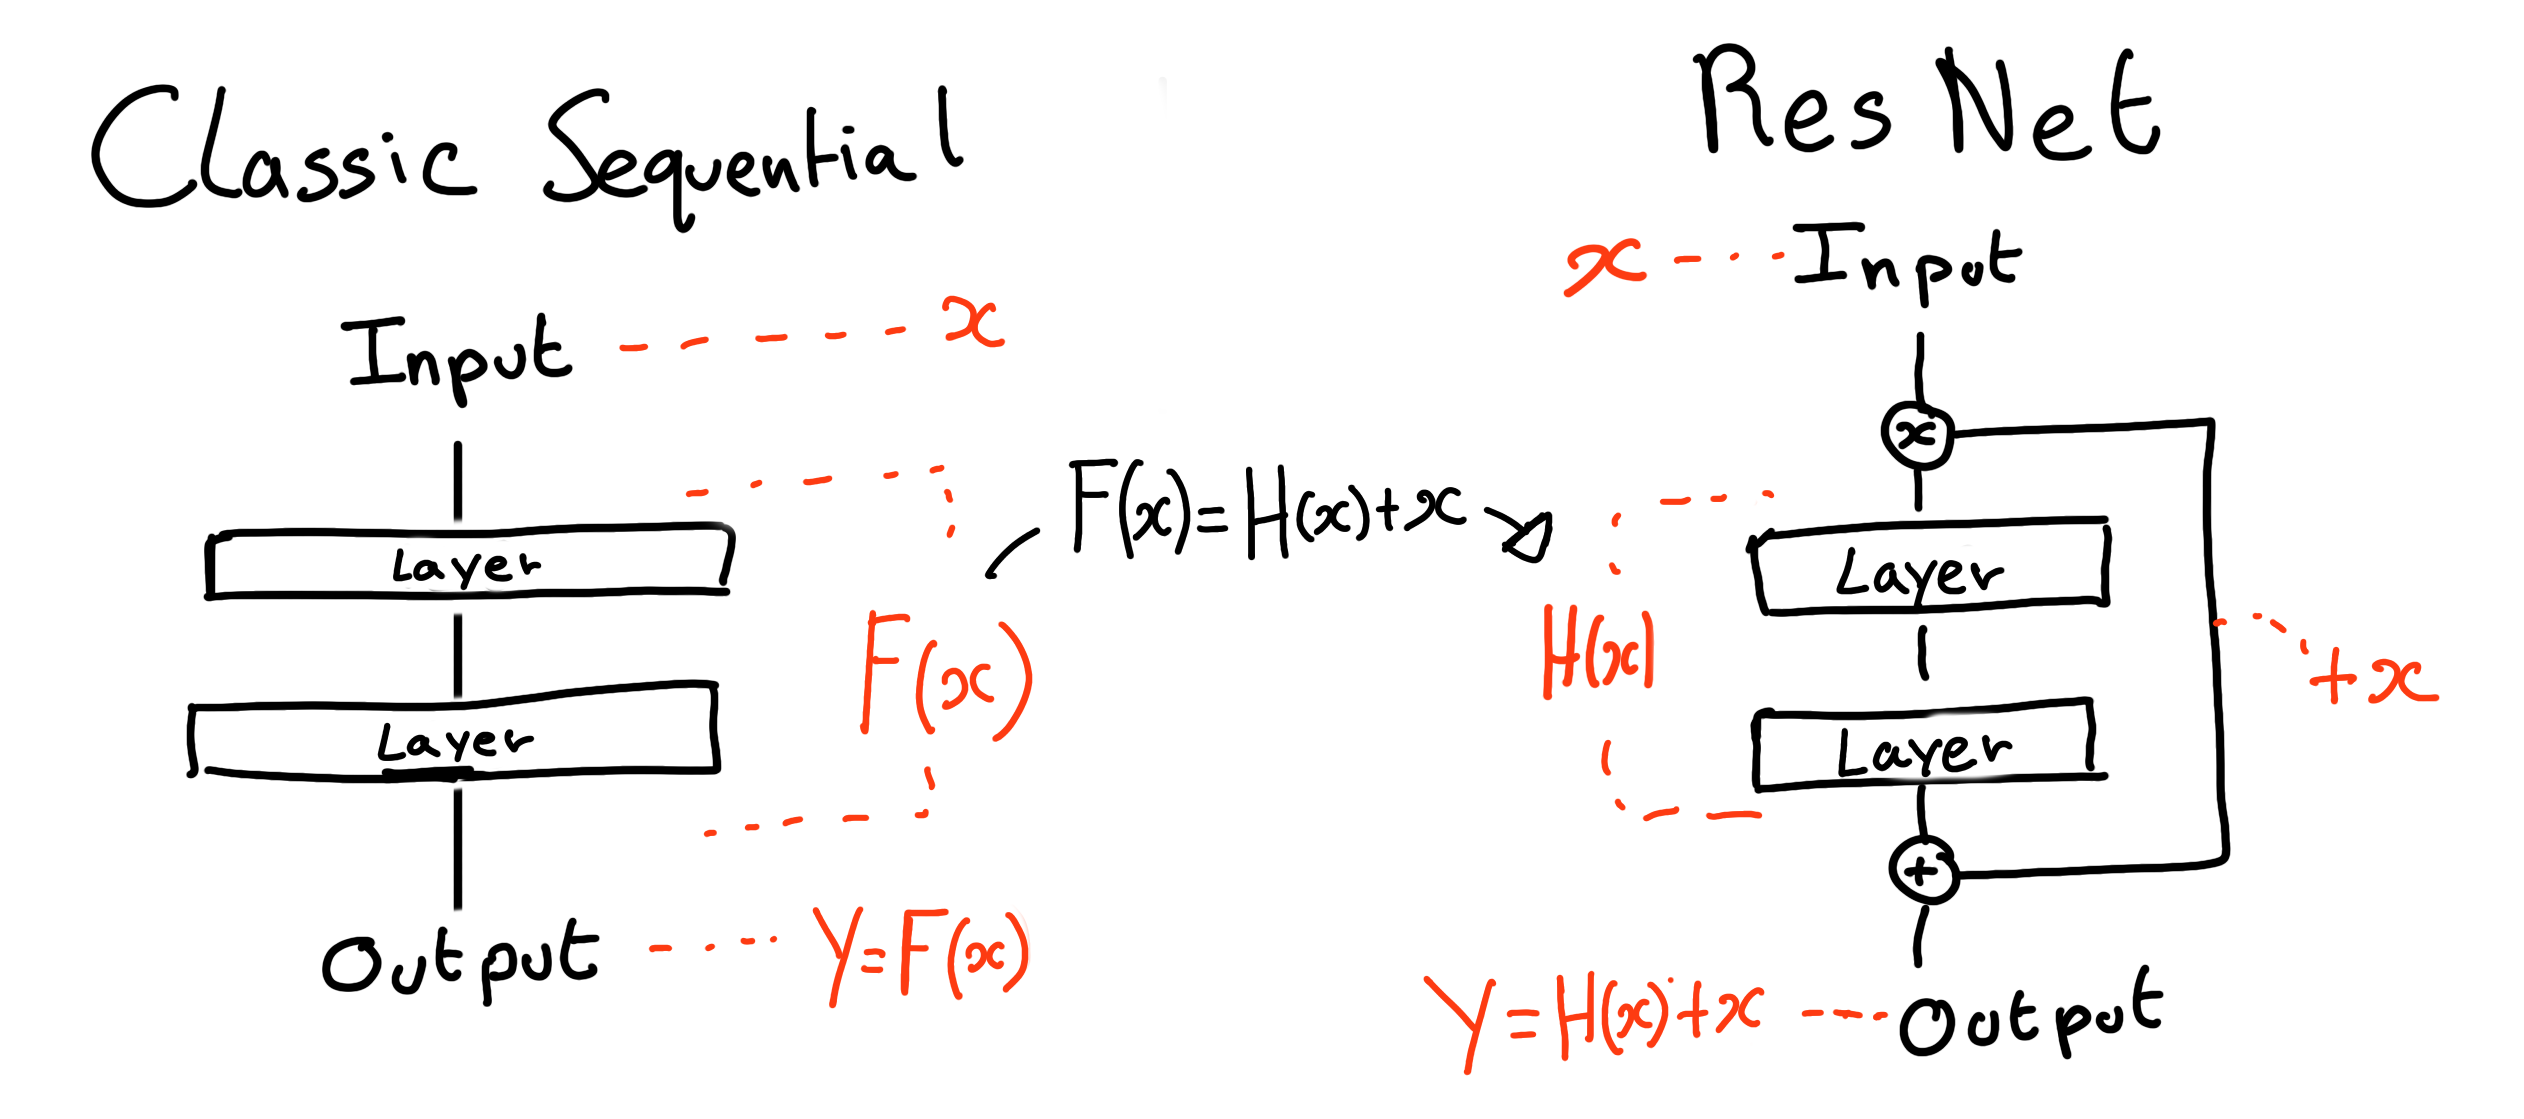
\includegraphics[height=6cm]{images/ml/resnet.png}
  \caption{Illustration of the ResNet framework}
  \label{fig:ml:resnet}
\end{figure}

\subsubsection{Gradient explosion}
Gradient explosion occurs when gradients grow exponentially during backpropagation, causing parameter values to increase dramatically. This is particularly problematic in deep networks where the product of large gradients across layers can lead to unstable updates. In practice, gradient explosion is often caused by large learning rates, poor weight initialization, or nonlinearities in the network.
For illustration, consider that the loss dependency in $\theta$ follow
\begin{align*}
  \mathcal{L}(\theta) &= \frac{\theta^2}{2} + e^{4\theta} \\
  \frac{\partial \mathcal{L}}{\partial \theta} &= \theta + 4e^{4\theta}
\end{align*}
The explosion is illustrated in Figure \ref{fig:ml:explosion} where we can see that the loss degrade with each step of optimization. In this illustration it is clear that reducing the learning rate suffice but this behaviour can happens in the middle of the training where the learning rate schedule does not permit reactivity.

There exist solutions to prevent this explosions:
\begin{itemize}
  \item \textbf{Gradient clipping}: Is this case we work on the gradient so that the norm of gradient vector does not exceed a certain threshold. In our illustration in Figure \ref{fig:ml:explosion} the gradient for $\theta > 0$ could be clipped at 3 for example.
  \item \textbf{Batch normalization}: For the same reasons as for gradient vanishing, normalizing the input data help reduce erratic behaviour.
\end{itemize}


\begin{figure}[ht]
  \centering
  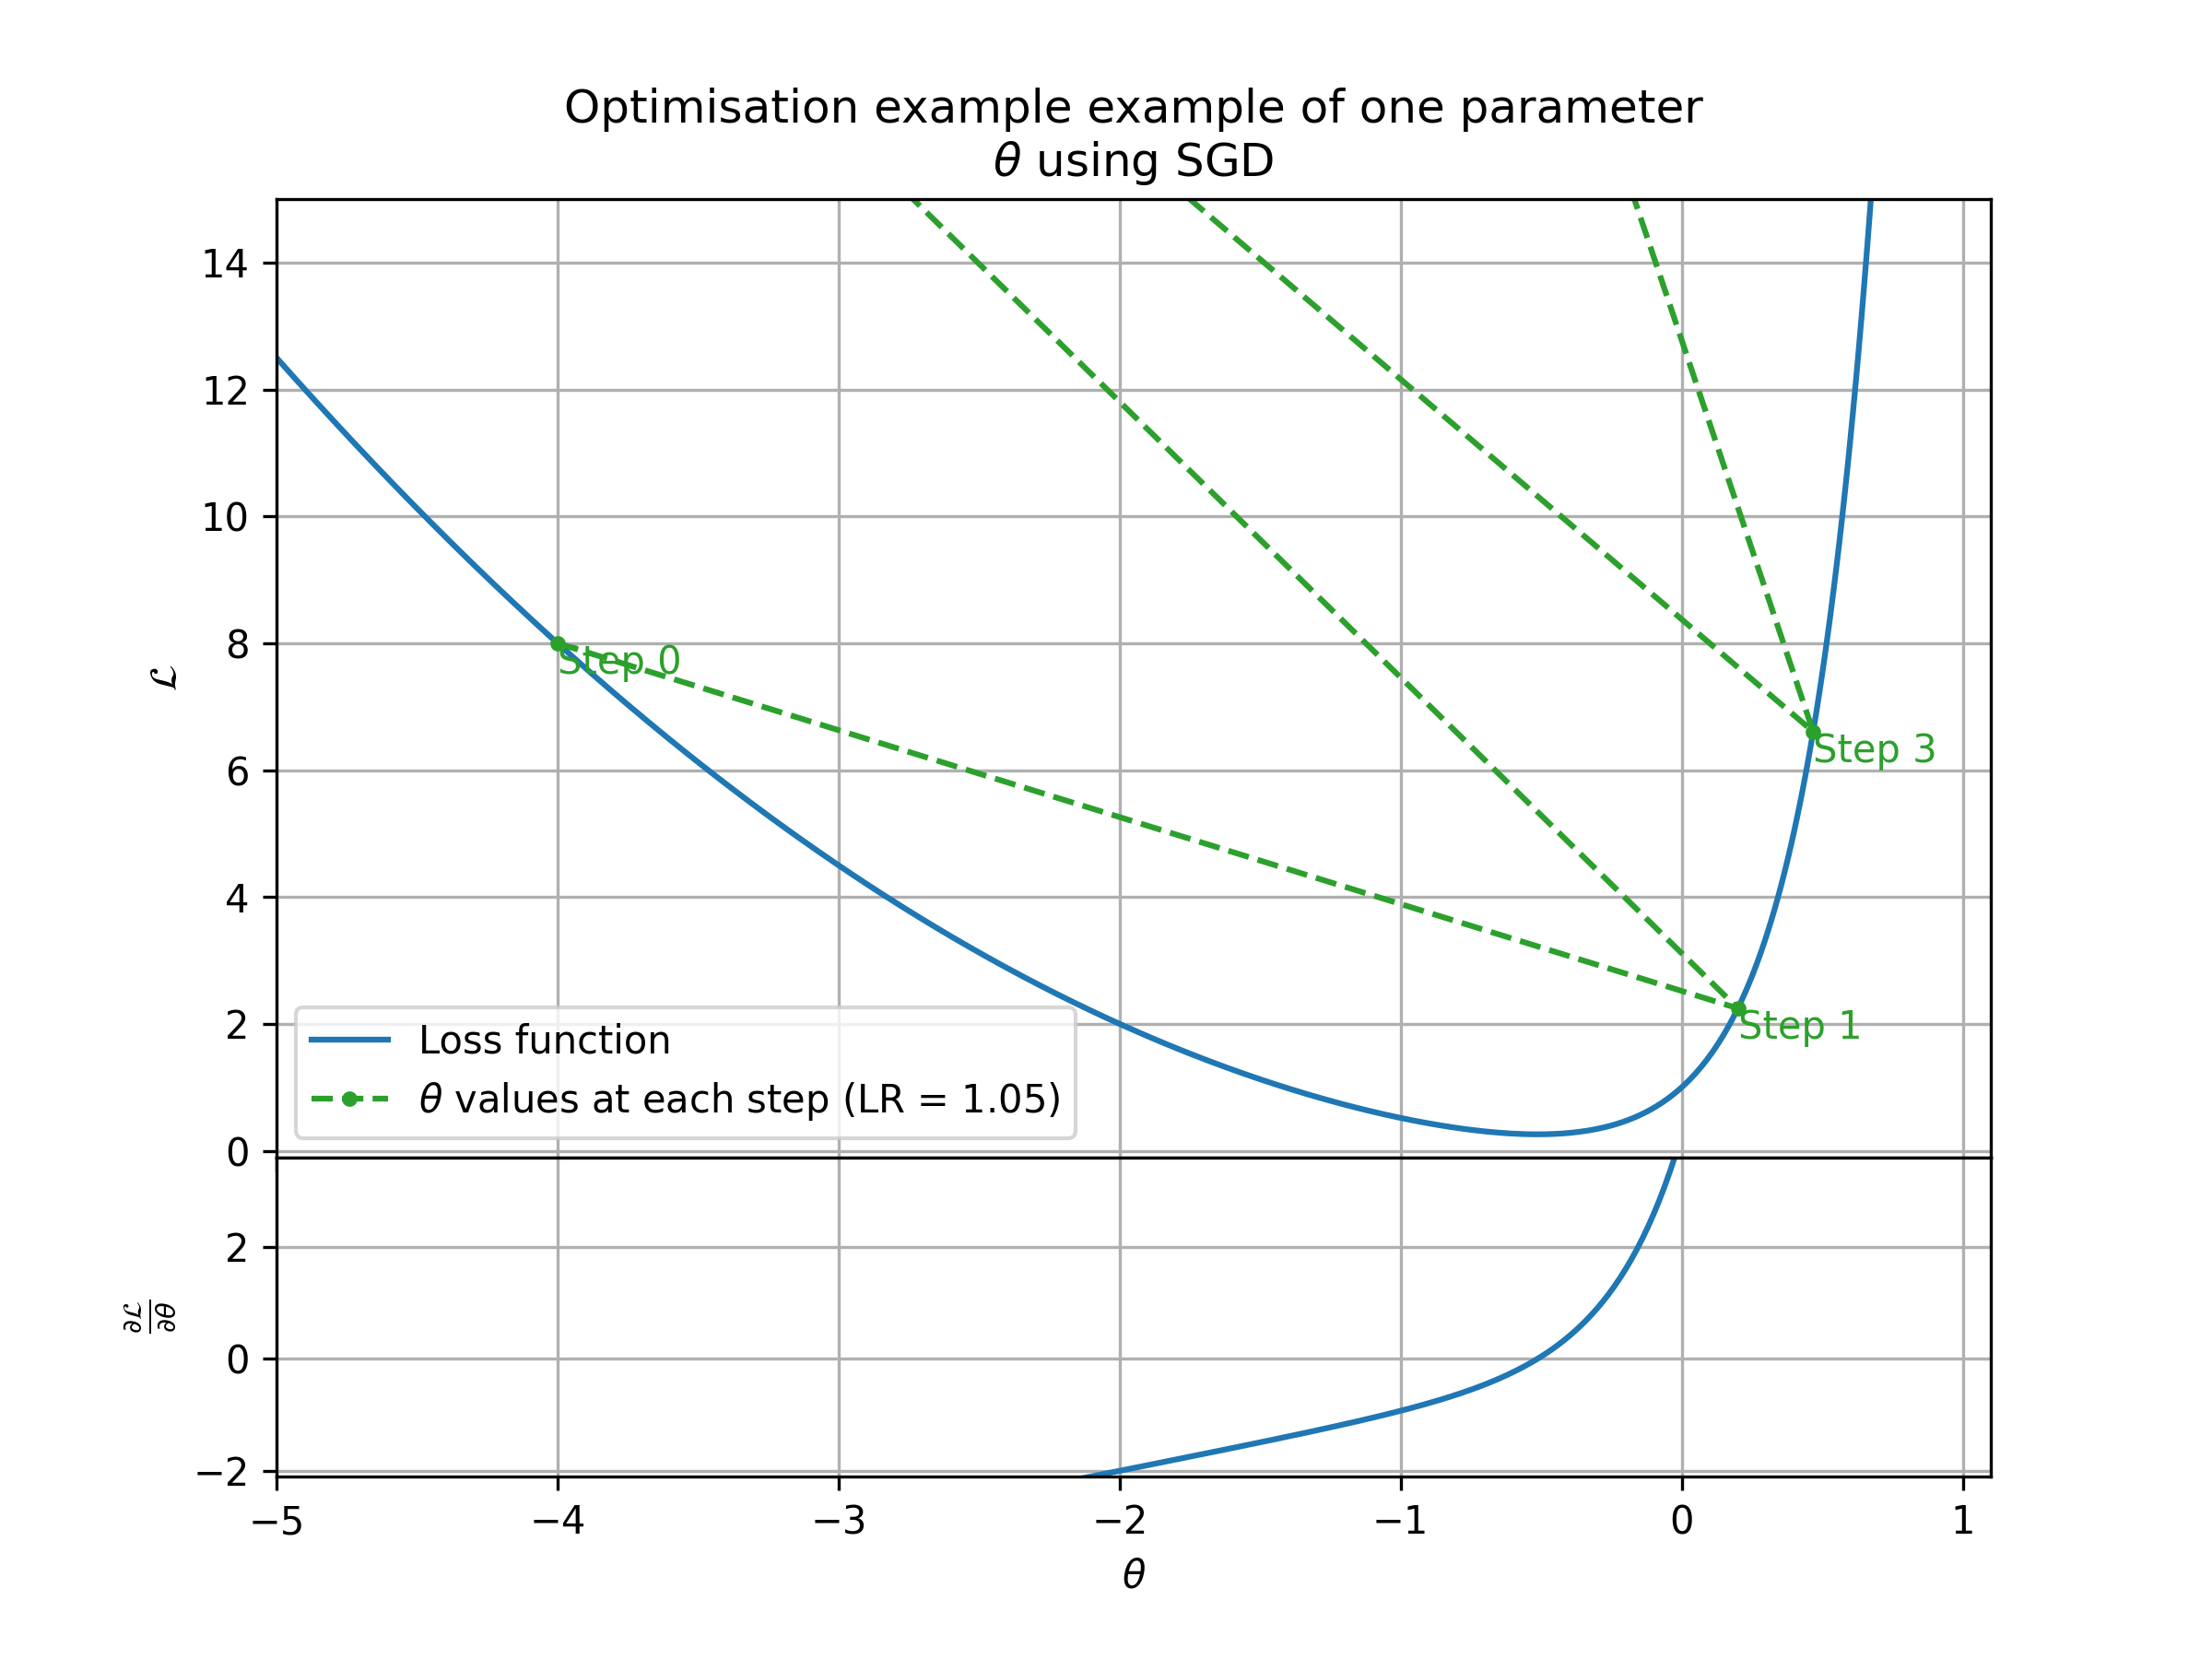
\includegraphics[height=6cm]{scripts/plots/MSE_explosion_illustration.png}
  \caption{Illustration of the gradient explosion. Here it can be solved with a lower learning rate but its not always the case.}
  \label{fig:ml:explosion}
\end{figure}


\section{Neural networks architectures}
\label{sec:ml:architecture}

\subsection{Fully Connected Deep Neural Network (FCDNN)}
\label{sec:ml:fcdnn}

In this thesis, FCDNN serves as a baseline architecture for comparison with more specialized models like CNNs (see Section \ref{sec:ml:cnn}) and GNNs (see section \ref{sec:ml:gnn}), which are better suited to structured or graph-based data. However, FCDNNs are still useful when modeling highly abstract relationships, such as aggregating features from the JUNO PMTs. While they are powerful, their main drawback lies in their inefficiency when dealing with high-dimensional or spatially structured data, which will be addressed with convolutional architectures.
This architecture is the stack of multiple fully connected layers as presented in the Figure \ref{fig:ml:fcdnn}. Most of the time, the classic ReLU function
\begin{equation}
  \label{eq:ml:relu}
  \mathrm{ReLU}(x) = \begin{cases}
    x & \mathrm{if} ~ x \geq 0 \\
    0 & \mathrm{otherwise}
  \end{cases}
\end{equation}
is used as activation function. Prelu and Sigmoid are also popular choices:


\begin{minipage}{0.5\linewidth}
  \begin{equation}
    \label{sec:ml:sigmoid}
    \mathrm{Sigmoid}(x) = \frac{1}{1+ e^{-x}}
  \end{equation}
\end{minipage}
\begin{minipage}{0.5\linewidth}
  \begin{equation}
    \label{sec:ml:prelu}
    \mathrm{PReLU}(x) = \begin{cases}
      x & \mathrm{if} ~ x \geq 0 \\
      \alpha x & \mathrm{otherwise}
    \end{cases}
  \end{equation}
\end{minipage}


The reasoning behind ReLU and PReLU is that with enough of them, you can mimic any continuous function as illustrated in Figure \ref{fig:ml:relu-mimic}. Sigmoid is more used in case of classification, its behavior going hand in hand with the Cross Entropy loss function used in classification problems.

\begin{figure}[ht]
  \begin{subfigure}[t]{0.48\textwidth}
    \centering
    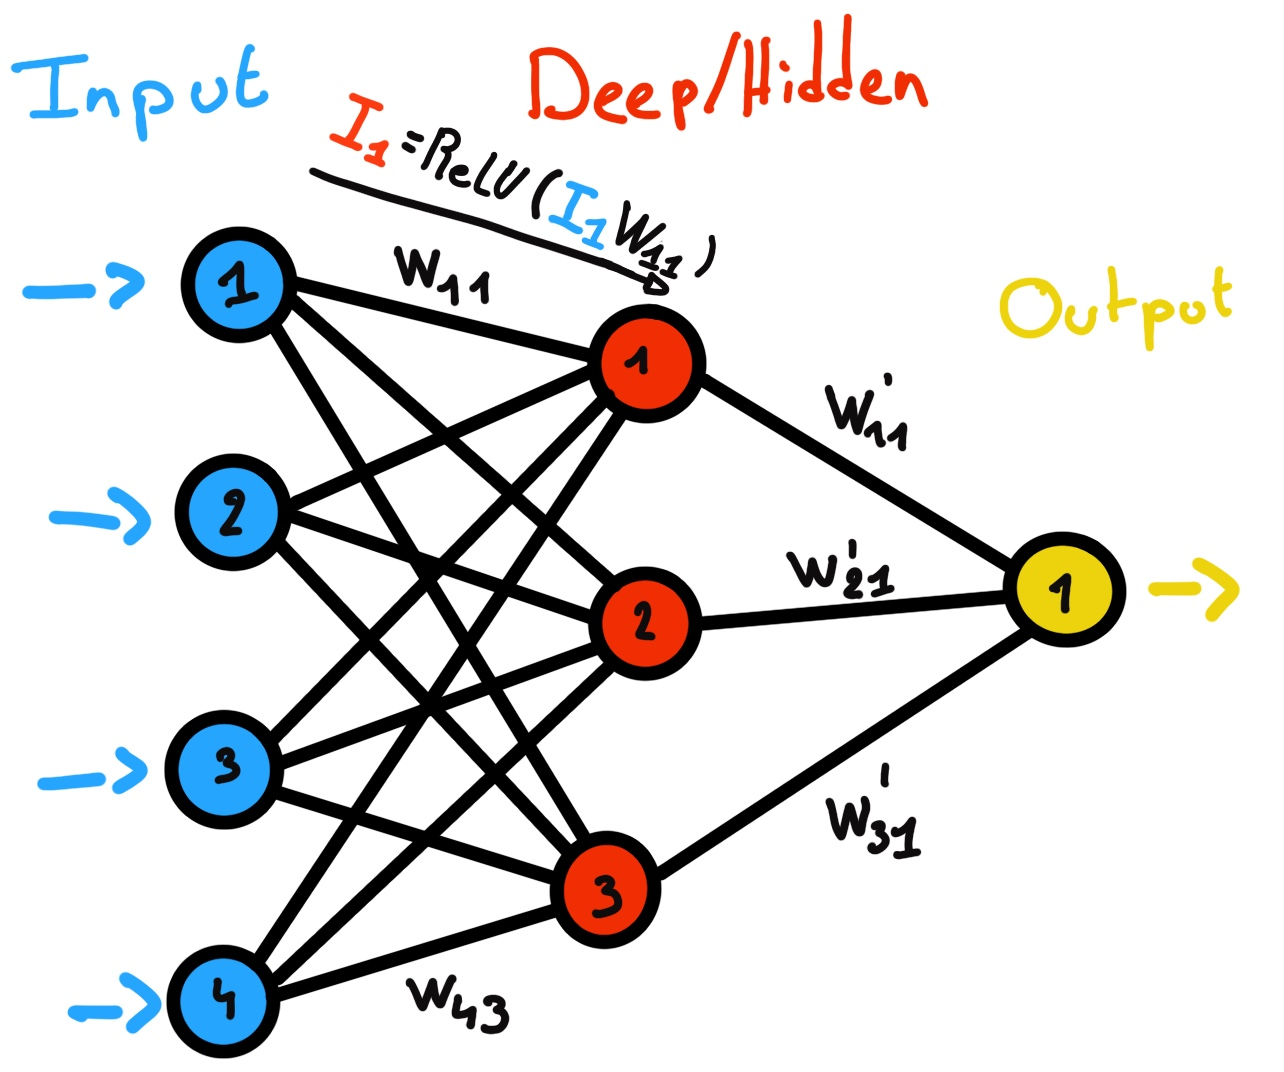
\includegraphics[height=6cm]{images/ml/fcdnn_scheme.jpg}
    \caption{Schema of a FCDNN}
    \label{fig:ml:fcdnn}
  \end{subfigure}
  \hfill
  \begin{subfigure}[t]{0.48\textwidth}
    \centering
    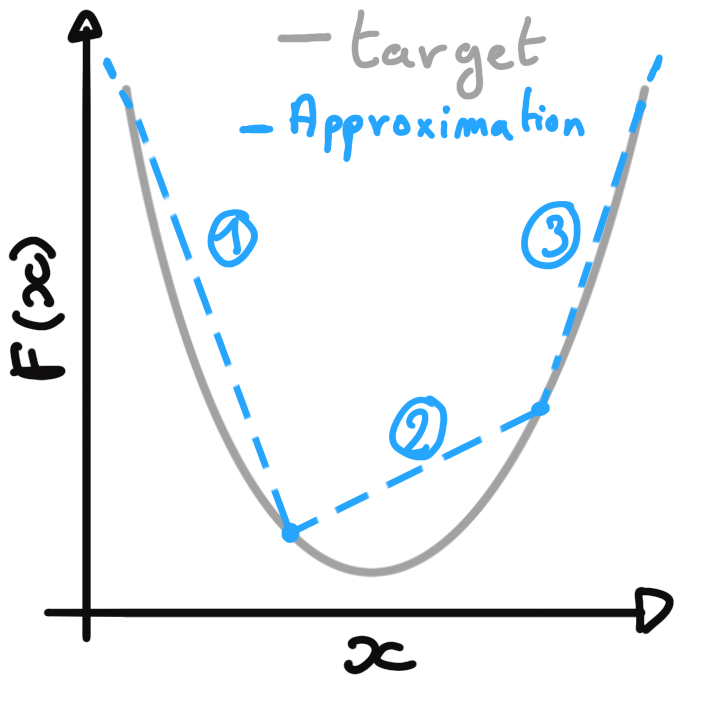
\includegraphics[height=6cm]{images/ml/relu_approx.png}
    \caption{Illustration of a composition of ReLU ``approximating'' a function. (1) No ReLU is taking effect (2) One ReLU is activating (3) Another ReLU is activating}
    \label{fig:ml:relu-mimic}
  \end{subfigure}
  \caption{}
\end{figure}

Due to its simplicity, FCDNN are also used as basic pieces for more complex architectures such as the CNN and GNN that will be presented in the next sections.

\subsection{Convolutional Neural Network (CNN)}
\label{sec:ml:cnn}

It's not trivial to describe in text the principles of Convolutional Neural Network (CNN) and how they works. We try a general description below followed by a step by step description of a concrete example.

Convolutional Neural Networks are a family of neural networks that use discrete convolution filters, as illustrated in an example in Figure \ref{fig:ml:conv_filter}, to process the input data, often images. They are commonly used in image recognition \cite{russakovsky_imagenet_2015} for classification or regression problematics. Concretely, you multiply element-wise a portion of the input data, in the case of an image, a small part of the image, with a kernel of same dimension. In Figure \ref{fig:ml:conv_filter}, we multiply the $3\times3$ pixels sub-image with the $3\times3$ kernel.

Their filters scan the input data, highlighting patterns of interest, this scanning procedure making them translation-invariant. In the concrete case of Figure \ref{fig:ml:conv_filter}, for each pixel of the input image, we group it with the 8 neighbours pixel and produce a new pixel that correspond to the output image. For the pixel on the edges that do not have neighbours, we either create ``imaginary'' pixel with the value 0 or we just ignore them. If we ignore them, the output image will posses fewer pixels than the input image. We see that the operation do not care where is the pattern of interest in the images, the filter output will be \textit{invariant} whatever \textit{translation} is applied to the image.

This invariance mean that they are capable of detecting oriented features independently of their location on the image.
These filters scan the input, highlighting important features like edges or textures, which in JUNO's case could represent spatial correlations in the timing and charge data across the detector. As the network goes deeper, it can capture more complex and abstract features, making it ideal for detecting nuanced particle interactions.
Again taking \ref{fig:ml:conv_filter} as an example, with only the 9 parameters composing the kernel, we can highlight the contour of the duck by looking at the ``yellowness'' of the pixels.

The learning parameters of CNNs are the kernels components, the network thus learn the optimal filters to extract the desired features.

The convolution layers are commonly chained \cite{simonyan_very_2015}, reducing the input dimension while increasing the number of filters. The idea behind is that the first layers will process local informations and the latest layers will process more global informations, as the latest convolution filters will process the results of the preceding that themself have processed local information. To try to preserve the amount of information, we tend to grow the numbers of filters for each division of the input data.
The results of the convolution filters is commonly then flattened and feed to a smaller FCDNN which will process the filters results to yield the desired output.

\begin{figure}[ht]
  \centering
  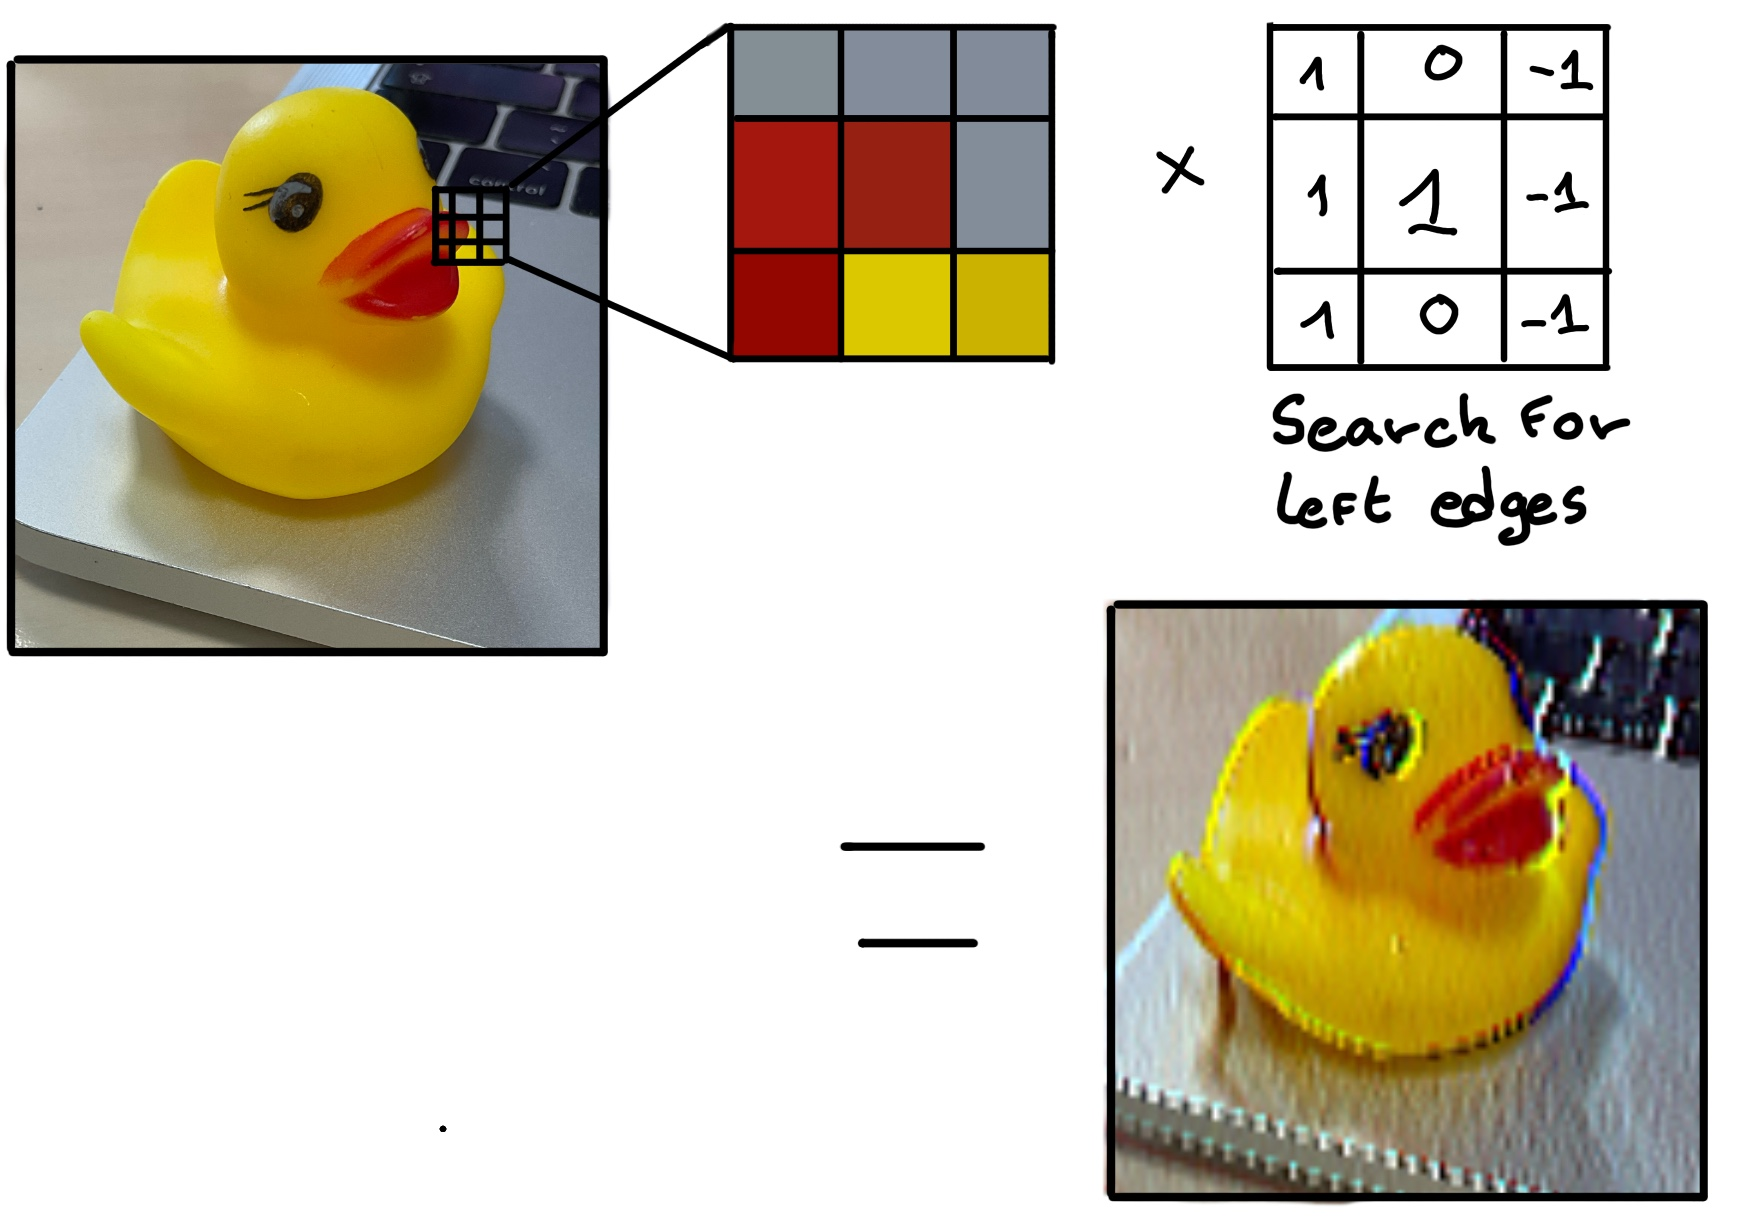
\includegraphics[height=6cm]{images/ml/convolution_exammple.jpg}
  \caption{Illustration of the effect of a convolution filter. Here we apply a filter with the aim do detect left edges. We see in the resulting image that the left edges of the duck are bright yellow where the right edges are dark blue indicating the contour of the object. The convolution was calculated using \cite{allen_generic-github-userimage-convolution-playground_2024}.}
  \label{fig:ml:conv_filter}
\end{figure}

As an example, let's take the Pytorch \cite{ansel_pytorch_2024} example for the MNIST \cite{lecun_gradient-based_1998}, a dataset of black and white images of handwritten digits. Those images are $28 \times 28$ pixels with only one channel corresponding to the grey level of the pixel. Example of images from this dataset are presented in Figure \ref{fig:ml:mnist}

A schema of the CNN used in the Pytorch example is presented in Figure \ref{fig:ml:cnn_mnist}. Using this schema as a reference, the trained network is made of:
\begin{enumerate}
  \item A convolutional layer of $(3 \times 3)$ filters yielding 32 channels. A bias parameter is applied to each channel for a total of $(32 \cdot (3\times3) + 32) = 320$ parameters. The resulting image is $(26\times26 \times 32)$ (26 per 26 pixels with 32 channels). The ReLU activation function is applied to each pixel.
  \item A second convolutional layer of $(3 \times 3)$ filters yielding 64 channels. This channel also posses a bias parameter for a total of $(64 \cdot (3\times3) + 64) = 640$ parameters. Resulting image is $(24\times24\times64)$. This channel also apply a ReLU activation function.
  \item Then comes a $(2\times2)$ max pool layer with a stride of 1 meaning that for each channel the max value of pixels in a $(2\times2)$ block is condensed in a single resulting pixel. The resulting image is $(12 \times 12 \times 64)$.
  \item This image goes through a dropout layer which will set the pixel to 0 with a probability of 0.25. This help prevent overtraining the neural network (see Section \ref{sec:ml:pitfall} for more details).
  \item The data is the flattened i.e. condensed into a vector of $(12 \times 12 \times 64) = 9216$ values.
  \item Then comes a fully connected linear layer (Eq. \ref{eq:ml:fully-connected}) with a ReLU activation that output 128 feature. It needs $(9216 \cdot 128)+ 128 = 1'179'776$ parameters.
  \item This 128 item vector goes through another dropout layer with a probability of $0.5$
  \item The vector is then transformed through a linear layer with ReLU activation. It output 10 values, one for each digit class (0, 1, 2, ..., 9). It need $(128 \cdot 10) + 128 = 1408$ parameters.
  \item Finally the 10 values are normalized using a log softmax function $\mathrm{LogSoftmax}(x_i) = \log \bigg(\frac{\exp(x_i)}{\sum_j \exp(x_j)}\bigg)$. Each of those values are the probability of the input image to be a certain digit.
\end{enumerate}

\begin{figure}[ht]
  \centering
  \begin{subfigure}[t]{0.48\linewidth}
    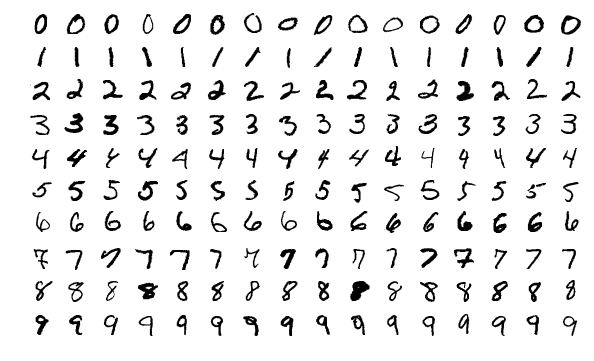
\includegraphics[width=\linewidth]{images/ml/MnistExamples.png}
    \caption{Example of images in the MNIST dataset}
    \label{fig:ml:mnist}
  \end{subfigure}
  \hfill
  \begin{subfigure}[t]{0.48\linewidth}
    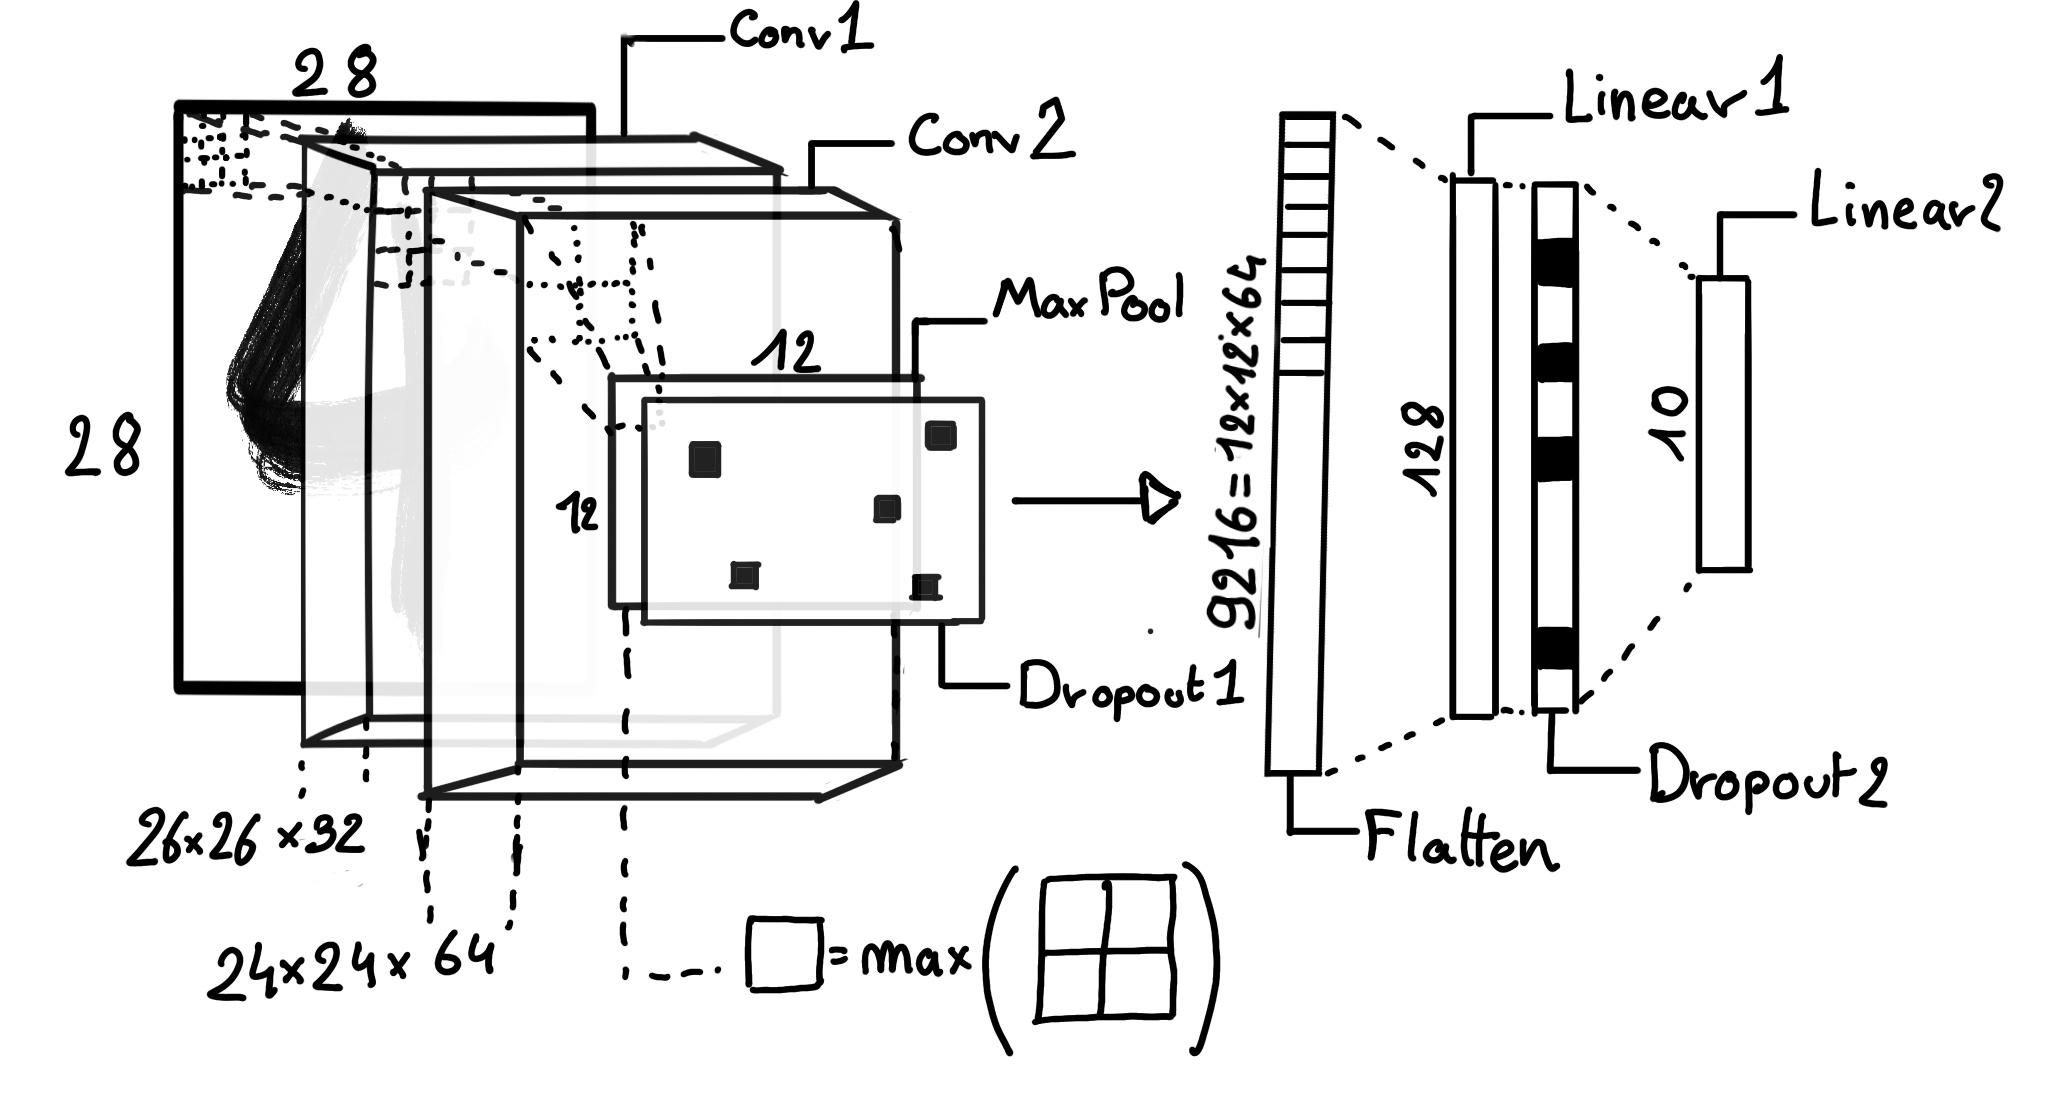
\includegraphics[width=\linewidth]{images/ml/mnist_cnn.jpg}
    \caption{Schema of the CNN used in Pytorch example to process the MNIST dataset}
    \label{fig:ml:cnn_mnist}
  \end{subfigure}
  \caption{}
\end{figure}

The final network needs 1'182'144 parameters or, if we consider each parameters to be a double precision floating point, 9.45 MB of data. To gives a order of magnitude, such neural network is considered ``simple'', train in a matter of minutes on T4 GPU \cite{noauthor_nvidia_nodate} (14 epochs) and reach an accuracy in its prediction of 99\%.


\subsection{Graph Neural Network (GNN)}
\label{sec:ml:gnn}

In GNNs, data is represented as nodes and edges in a graph, which allows us to model the JUNO detector as a network of PMTs, where each PMT is a node and the edges represent relationships such as spatial distance or timing correlations between PMTs. This flexibility enables GNNs to capture complex interactions across the detector geometry that would be difficult to represent with a CNN. Furthermore, GNNs excel at processing non-Euclidean data, making them a natural fit for the irregular layout of the PMTs in JUNO.
In this thesis, GNNs are applied to model the spatial and temporal relationships between PMTs, enabling more precise event classification and reconstruction. By leveraging the message-passing framework, the GNN can aggregate information from neighboring PMTs, allowing it to detect subtle patterns in the detector's data.

To get deeper in details, we have seen in the previous section, the CNNs are powerful for image processing, and more generally any data that can be expressed as a regular, discrete space and from which the information reside in the dispersion in this space. For an image, the edges of an object and how they assemble. A red square, straight edges with a sharp angle between them, is much less representative of a duck than an yellow sphere, round edges without sharp angles.

This ``image'' projection is not fitted for every problematics. The signals produced by a detector does not always have the properties of images. In the case of JUNO for example, we can create an image of two channels, one for the charge $Q$ and one for the timing $t$ but this image should be spheric. Furthermore JUNO is by nature inhomogeneous, using two different systems : The LPMT and the SPMT. Those two systems have different regime, and thus should be processed differently. We could imagine images with four channels, two for the LPMT and two for the SPMT, or even a branched CNN with one convolution branch for the LPMT and another one for the SPMT. Anyway, the CNN will need to combine the two systems.

To get around the restrictions of data representation imposed by CNNs, we can use the more flexible \textit{graph} representation.
\begin{figure}[ht]
  \centering
  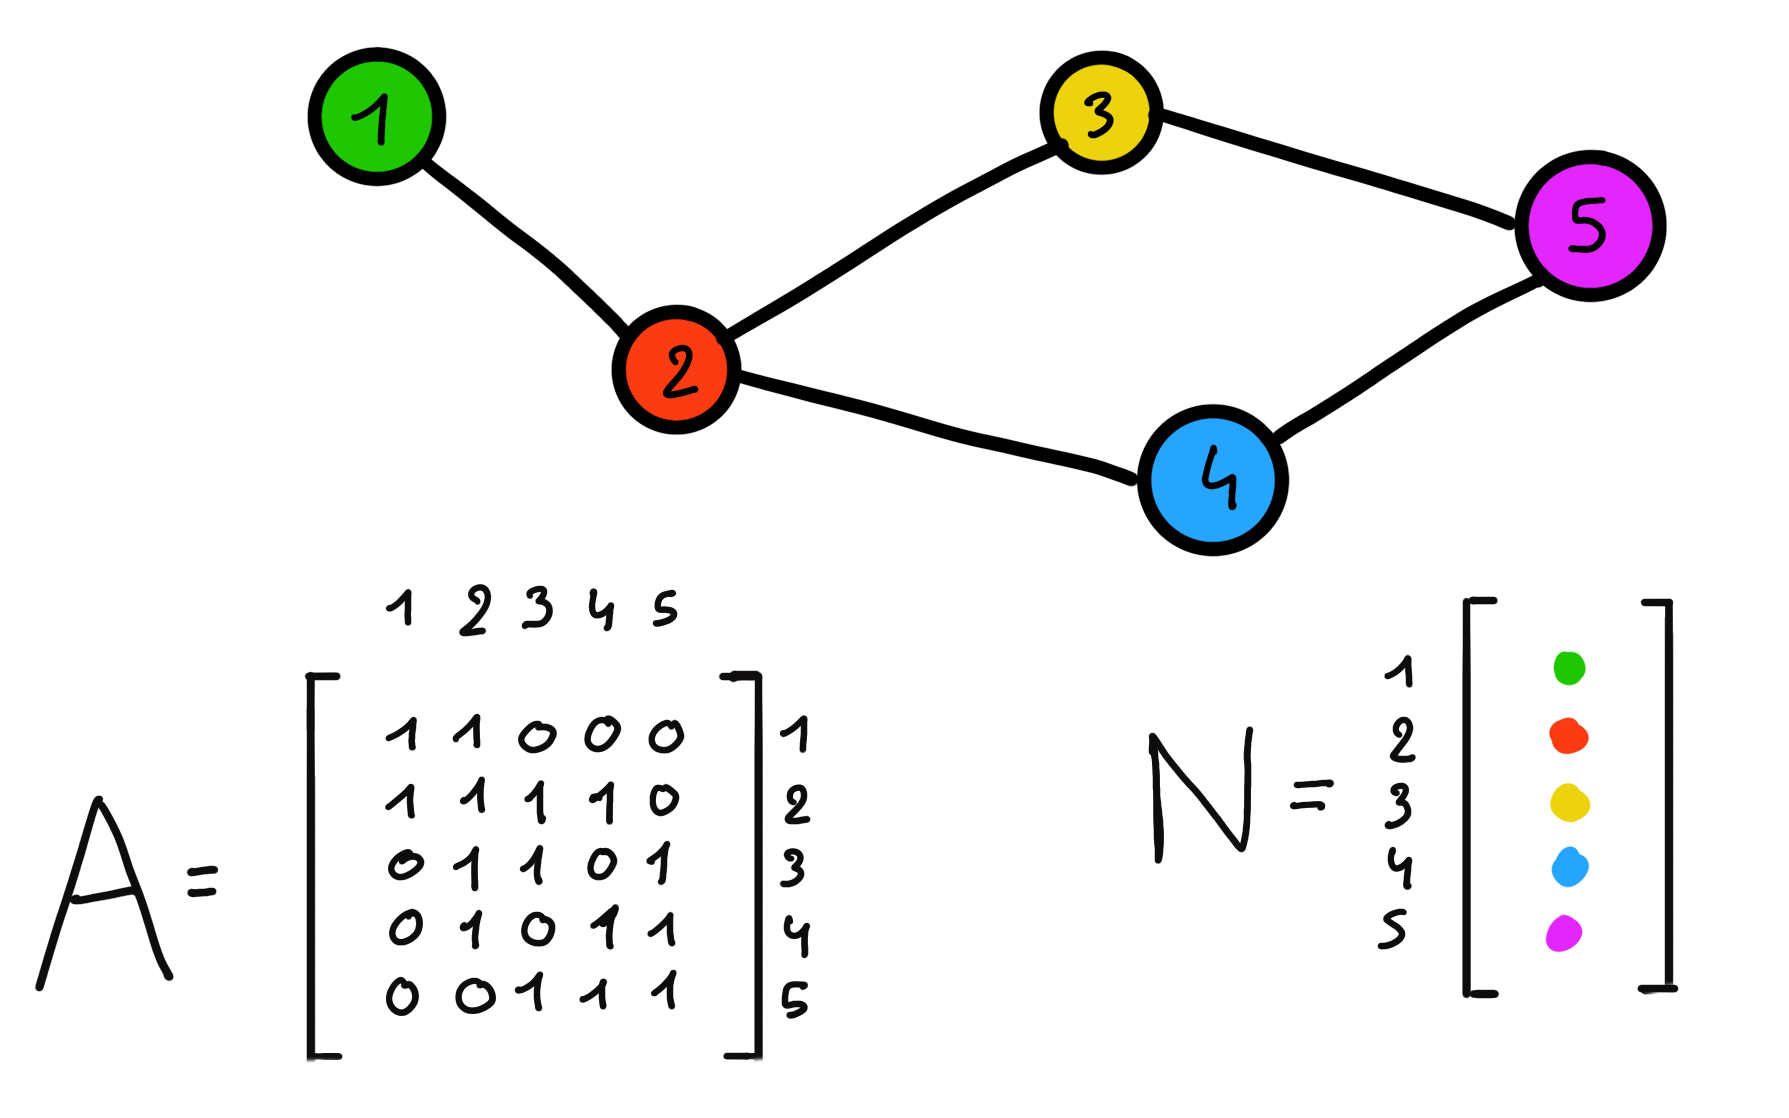
\includegraphics[height=6cm]{images/ml/graph_illustration.png}
  \caption{Illustration of a graph and its tensor representation.}
  \label{fig:ml:gnn:graph}
\end{figure}
A graph $G(\mathcal{N},\mathcal{E})$ is composed of vertex or node $n \in \mathcal{N}$ and edges $e \in \mathcal{E}$. The edges are associated to two nodes $(u, v) \in \mathcal{N}^2$, ``connecting'' them. The node and the edges can hold features, commonly represented as vector $n \in \mathbb{R}^{k_{n}}$, $e \in \mathbb{R}^{k_{e}}$ with $k_n$ and $k_e$ the number of features on the nodes and edges respectively. We can thus define a graph using two tensors $A^{ij}_{\epsilon}$ the adjacency tensor that hold the features $\epsilon \in [0, k_e]$ of the edge connecting the node $i$ and $j$ and the tensor $N^{i}_{\nu}$ that hold the features $\nu \in [0, k_n]$ of a node $i$.

More figuratively, using the example in Figure \ref{fig:ml:gnn:graph}, we have a graph of 5 nodes with a color as feature. The edges have no features, we thus encode their existences as 0 or 1. In a realistic examples as JUNO we could represent each PMTs as nodes and the edges between them as their relation such as distance, timing difference, etc... There no strict rules about what is a node or how they should be linked together. This abstraction allow us to represent virtually any type of detector of any geometry.

\begin{figure}[ht]
  \centering
  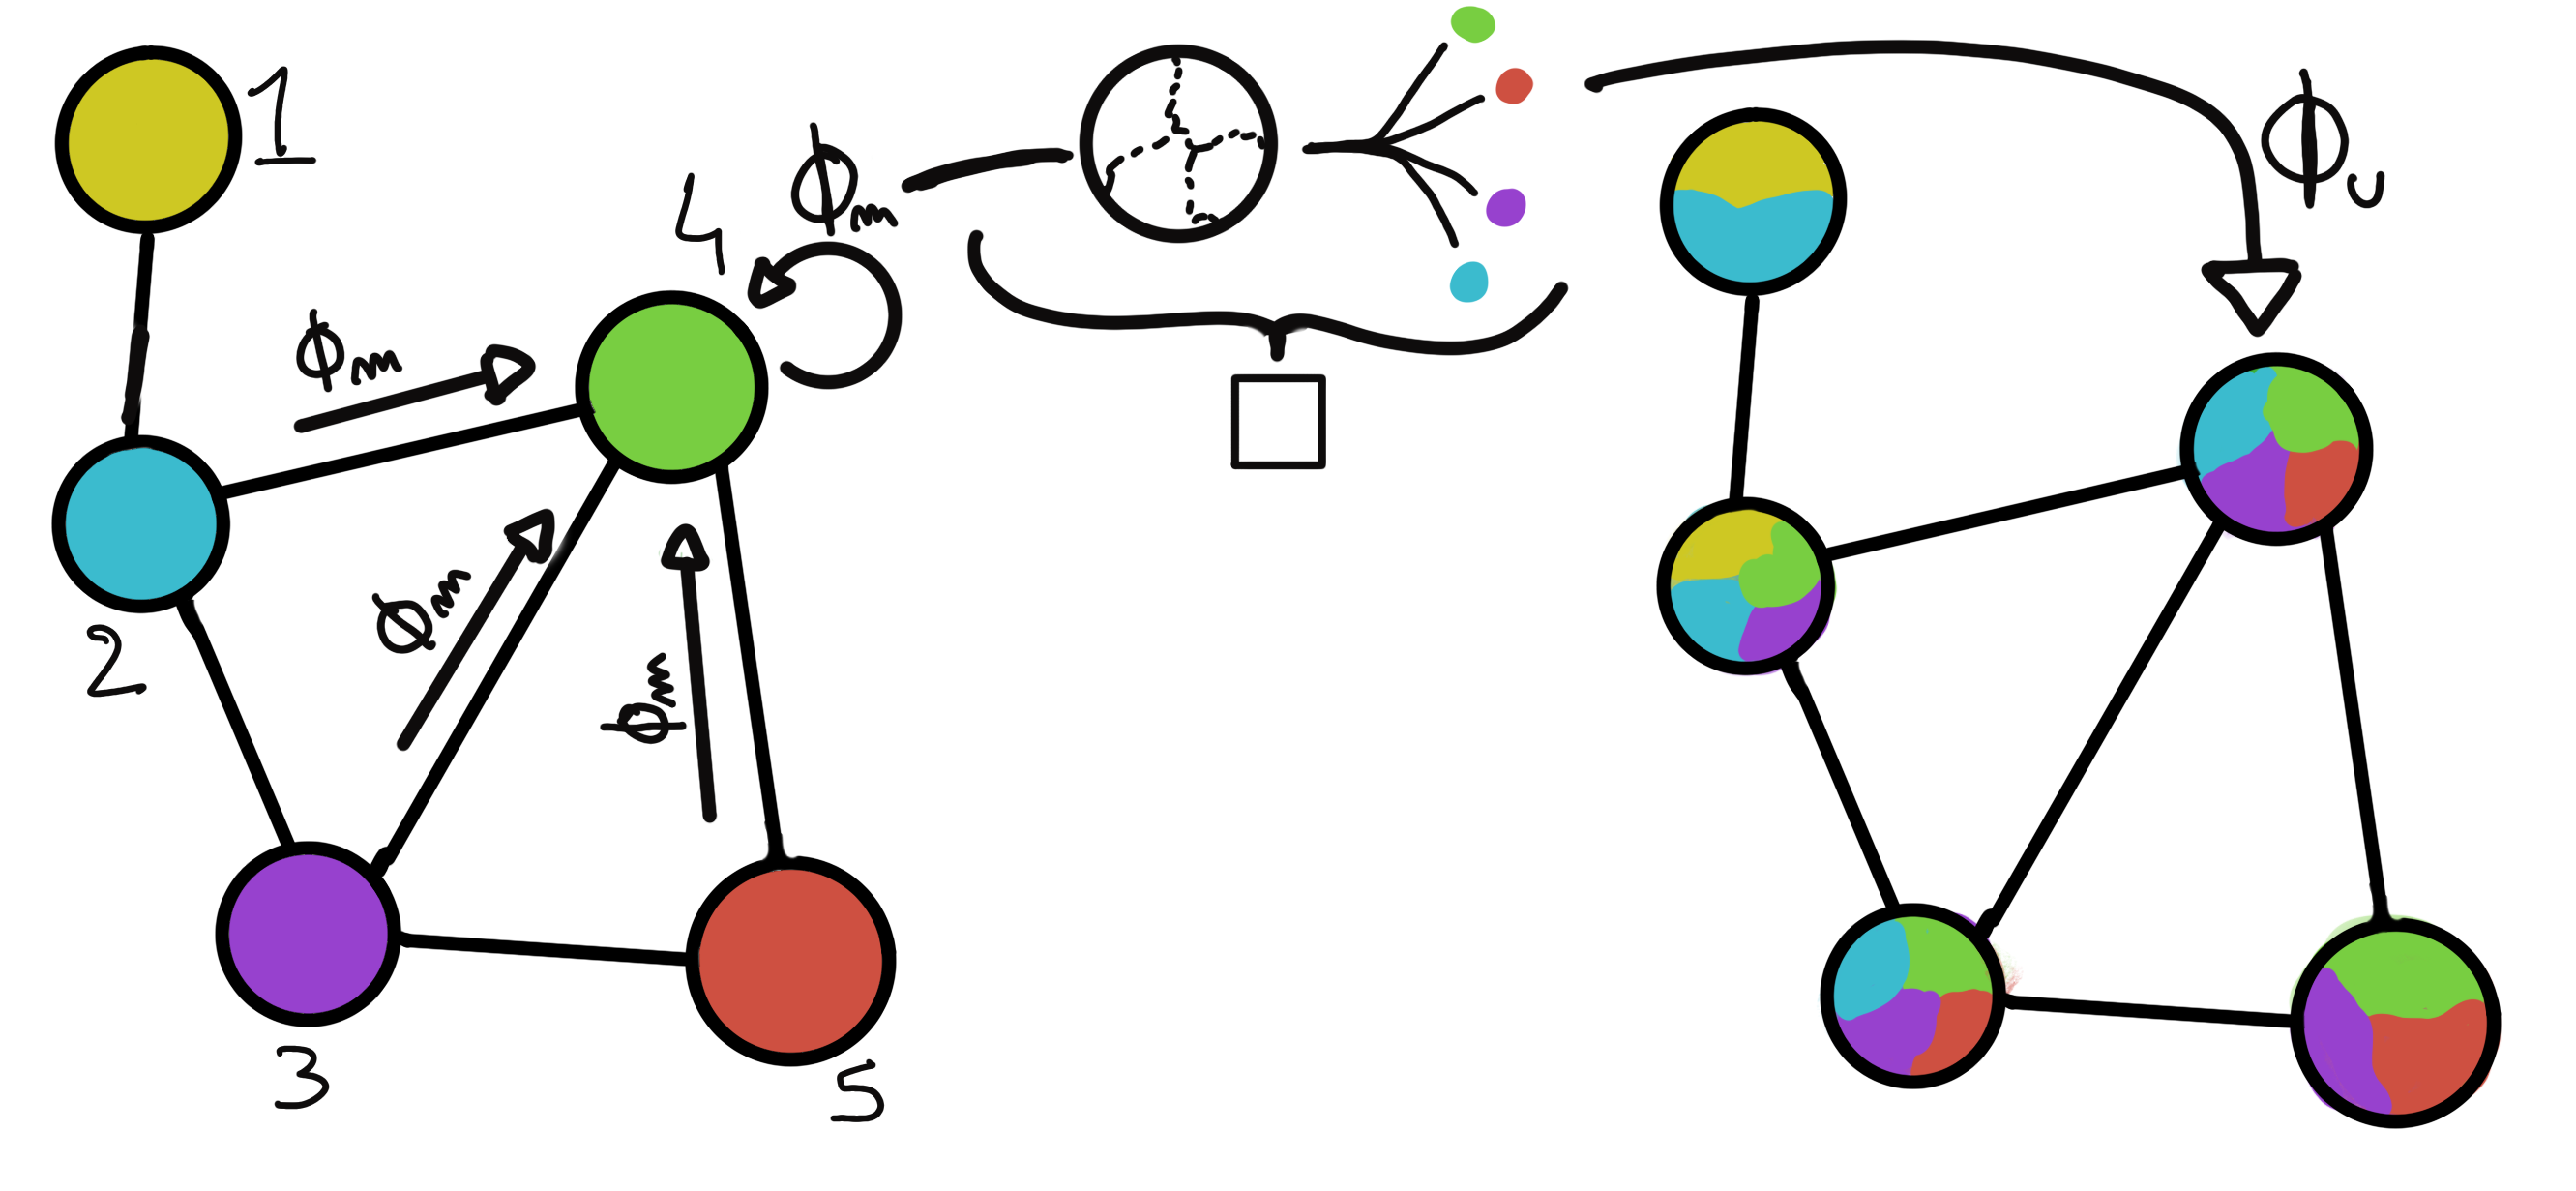
\includegraphics[height=6cm]{images/ml/message_passing.png}
  \caption{Illustration of the message passing algorithm. The detailed explanation can be found in Section \ref{sec:ml:gnn}}
  \label{fig:ml:gnn:message_passing}
\end{figure}

To process such object we need specific machine learning algorithms we call Graph neural network.
To efficiently manipulate graph we need to structurally encode their property in the neural network computing architecture: each node is equivalent (as opposite to ordered data in a vector), each node has a set of neighbours, ... One of this method is the message passing algorithm presented historically in ``Neural Message Passing for Quantum Chemistry'' \cite{gilmer_neural_2017}. In this algorithm, with each layer of message passing a new set of features is computed for each node following
\begin{equation}
  n_i^{k+1} = \phi_u (n_i^k, \Box_j \phi_m(n_i^k, n_j^k, e^k_{ij})); ~ n_j \in \mathcal{N}'_i
\end{equation}
where $\phi_u$ is a differentiable \textit{update} function, $\Box_j$ is a differentiable \textit{aggregation} function and $\phi_m$ is a differentiable \textit{message} function. $\mathcal{N}'_i = \{n_j \in \mathcal{N} | (n_i, n_j) \in \mathcal{E}\}$ is the set of neighbours of $n_i$, i.e. the nodes $n_j$ from which it exist an edge $e_{i,j} \rightarrow (n_i, n_j)$. $k$ is the layer on which the message passing algorithm is applied. The update function need also a few other property if we want to keep the graph property, most notably the permutational invariance of its parameters (example: mean, std, sum, ...). The differents message, update and aggregation functions can really be any kind of function if they follow the constraint presented before, even small Neural Network.

The edges features can also be updated, either by directly taking the results of $\phi_m$ or by using another message function $\phi_e$.

To explain this process, let's take the situation presented in Figure \ref{fig:ml:gnn:message_passing}. We start with an input graph on left, in this case the message passing algorithm is mixing the color on each nodes and produce nodes of mixed color. For simplicity, the $\phi_m$ and $\phi_u$ function are the identity, they take a color and output the same color.

Let's look at what's happening in the node 4. It has 3 neighbours and is a neighbour of itself. The four resulting $\phi_m$ extract the color of each nodes and then feed them to the $\Box$ function. The $\Box$ function just equally distribute the color in the node. Finally the $\phi_u$ function just update the node with the output of $\Box$.

Interestingly we see that the new node 4 does not have any yellow, the color of node 1. But if we were to run the message passing algorithm again, it would get some as node 2 is now partially yellow. If color here represent information, we see that multiple step are needed so that each node is ``aware'' of the informations the other nodes possess.


Message passing is a very generic way of describing the process of GNN and it can be specialized for convolutional filtering \cite{defferrard_convolutional_2017}, diffusion \cite{li_diffusion_2018} and many other specific operation. GNN are used in a wide variety of application such as regression problematics, node classification, edge classification, node and edge prediction, ...


It is a very versatile but complex tool.

\subsection{Adversarial Neural Network (ANN)}

The adversarial machine learning, Adversarial Neural Networks (ANN) in the case of neural network, is a family of unsupervised machine learning algorithms where the learning algorithm (generator) is competing against another algorithm (discriminator). Taking the example of Generative Adversarial Networks, concept initially developed by Goodfellow et al. \cite{goodfellow_generative_2014}, the discriminator goal is to discriminate between data coming from a reference dataset and data produced by the generator.
The generator goal, on the other hand, is to produce data that the discriminator would not be able to differentiate from data from the reference dataset. The expression of duality between the two models is represented in the loss where, at least a part of it, is driven by the results of the discriminator.

\end{document}
